\section{System architecture}
The core idea of the proposed solution is to implement a part of the system both in the guest and in the hypervisor, to combine the best features of the two approaches. To achieve this, the monitoring code must run inside the guest, so that it is possible to have access to the semantic information of the guest operating system itself. Certainly, there is the need to protect the part of the system running in the guest, otherwise, like already mentioned, it becomes an easy target for attackers, and this is done by the hypervisor.
\par
The overall system is based on the assumption that an attacker cannot deactivate the part of the system implemented in the hypervisor. This is a reasonable assumption because virtualization technologies have to provide isolation by design. However, in the past, attackers managed to escape from the guest virtual machine, gaining arbitrary code execution on the hypervisor's side. This kind of attack is often referred to as VM escape. In such a case, not only the monitoring system can be compromised, but also other virtual machines and the host itself. An example of these kinds of attacks can be found in CVE-2015-3456 \cite{venom-cve}, an exploit commonly known as VENOM, which allowed an attacker to execute code with the privileges of the QEMU process. It has been noticed that most of these kinds of attacks exploit bugs related to the I/O emulation service of QEMU, and recently, to prevent them, it has been proposed a multi-process version of QEMU, instead of the current monolithic one. The idea is to completely separate the services for I/O, having one process for each emulated device. This allows to introduce security measures with finer granularity: for instance, if a process is used to emulate a disk device, the set of the system calls it can use can be reduced using the \texttt{seccomp} system call and it can be forced to access only a limited set of files, i.e the disk image file and a few more, by using a Mandatory Access Control system (AppArmor, SELinux). An attacker escaping a VM and gaining the privileges of such a secured process cannot compromise the host system and other VMs with the same ease as in the monolithic version. The multi-process QEMU would only introduce benefits also for the proposed system, making its assumption even more reasonable. 
\par 
The system has to fulfill the following requirements:
\begin{enumerate}
    \item The monitoring code has to be executed in the guest at given time intervals, and the start of its execution must be ensured by the hypervisor.
    \item An attacker must not be able to prevent the execution of the monitoring code and cannot predict when its execution starts.
    \item The overall system must be designed with a defense in depth approach in mind. 
\end{enumerate}
\begin{figure}
\centering
  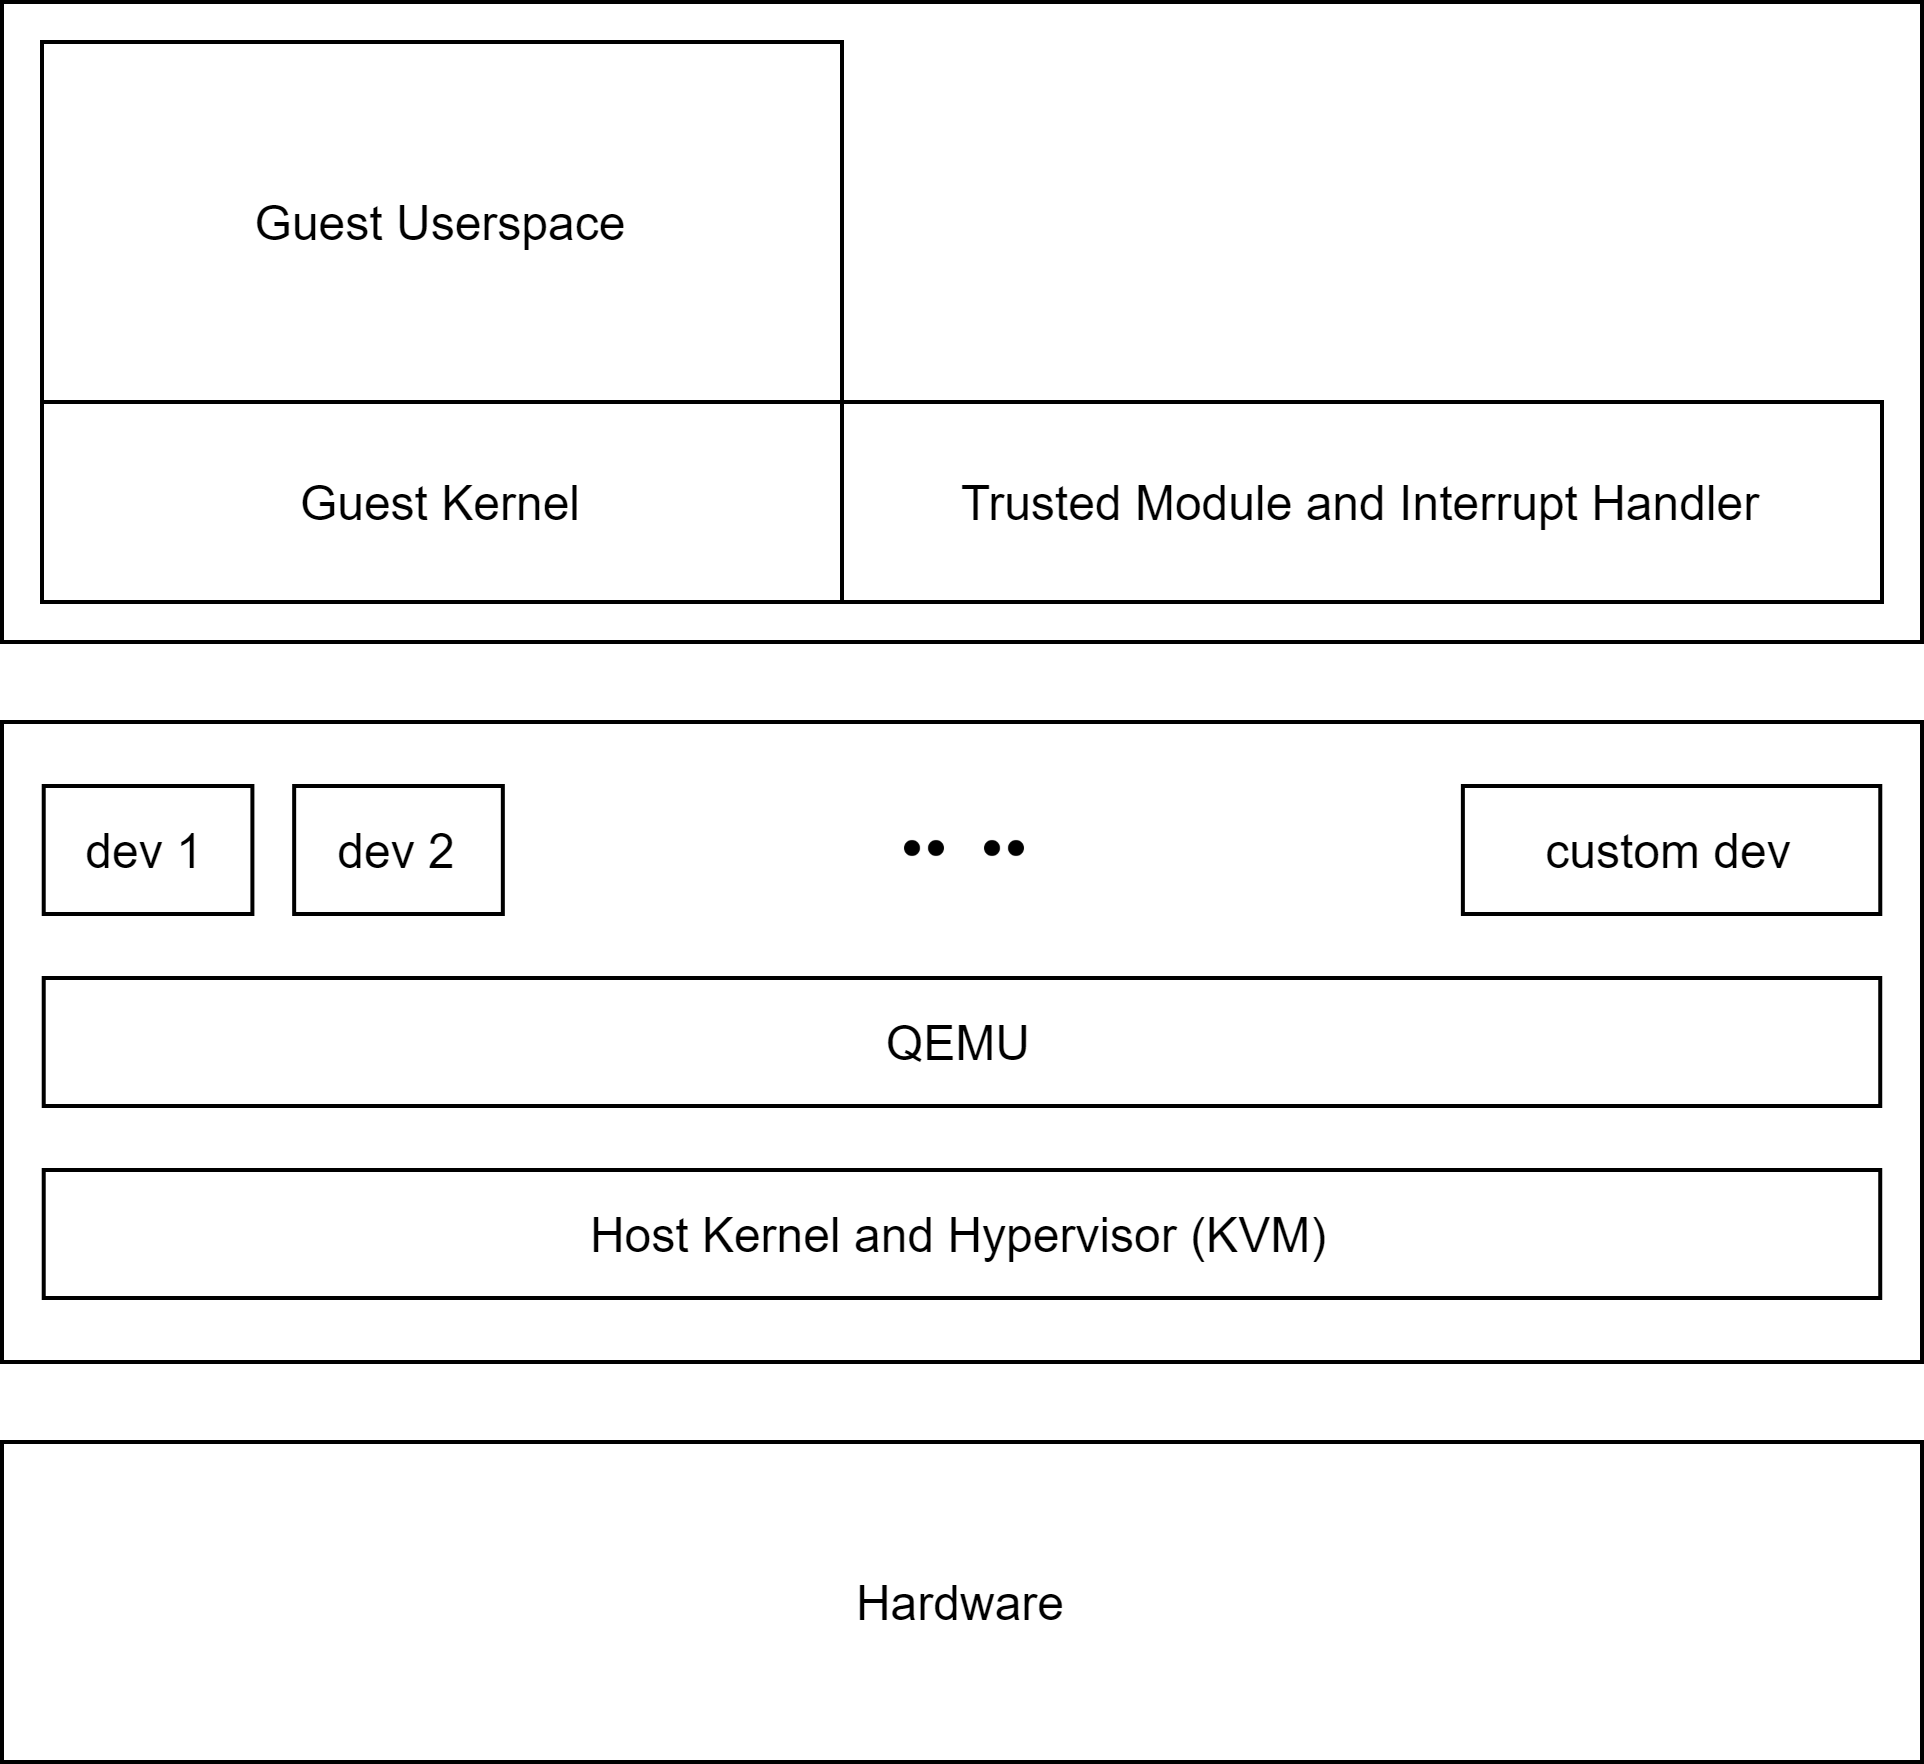
\includegraphics[scale=1]{images/sys-arch.png}
  \caption{Overall system architecture. }
  \label{fig:system-architecture}
\end{figure}
The system's architecture is illustrated in Figure \ref{fig:system-architecture} and aims at meeting these requirements.
\par
One way to fulfill them is by leveraging the interrupt handling mechanism. In fact, a custom virtual device is added to the QEMU source code and an interrupt handler is installed inside the guest thanks to a Loadable Kernel Module. This module is inserted in the system when it is considered to be in a safe state, e.g just after its boot and right before starting any network activities. The interrupt handler is responsible for encapsulating the monitoring code. It gets executed whenever the virtual device sends an interrupt, thus forcing the kernel to stop the actions that it was performing and executing the routine associated with the interrupt. Furthermore, the injection of the interrupt is completely up to the hypervisor, which can decide when to inject it regardless of what it is happening in the guest. 
\par
The hypervisor is also responsible for protecting the monitoring code inside the guest. In particular, it must take maximum effort to protect the interrupt handling mechanism in the Linux kernel, including code and data structures. To do that, it can both prevent the guest to write to important kernel objects or restore their state just before the injection of the interrupt, so that a certain degree of stealthiness is reached.
\begin{figure}[t]
    \centering
    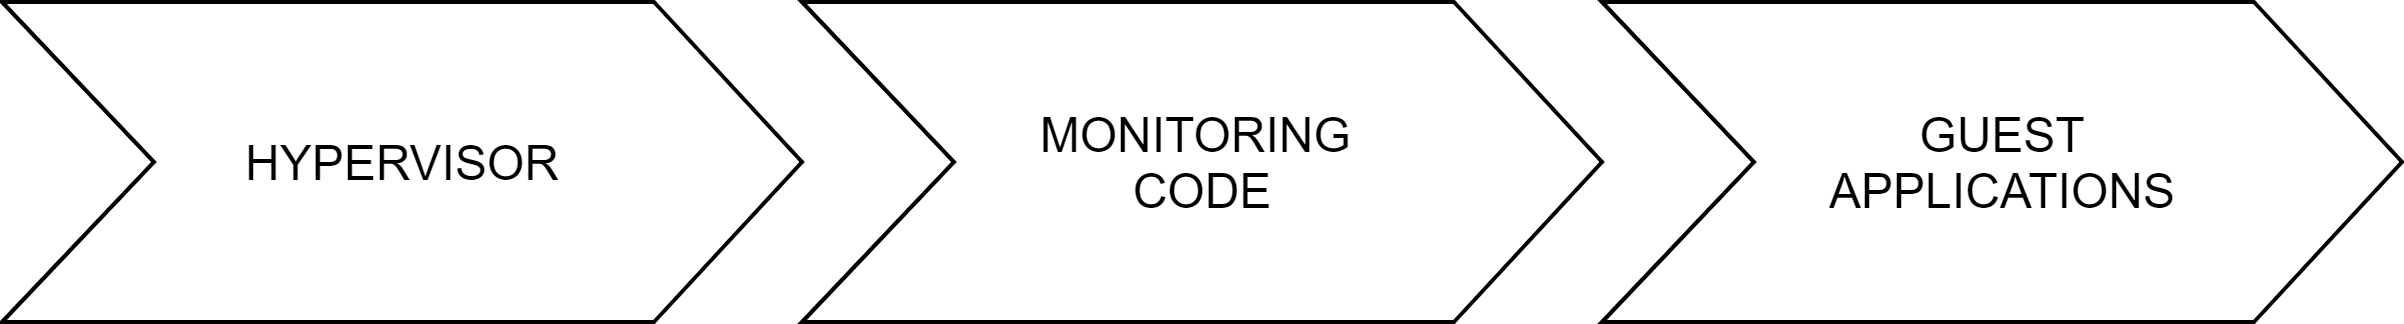
\includegraphics[width=\textwidth]{images/defense-in-depth.png}
    \caption{The defense in depth approach.}
    \label{fig:defense-in-depth}
\end{figure}
\par
The Stealthiness of the system is one of the many defenses that the system has to put in place. The proposed system tries to comply with a defense in depth approach like depicted in Figure \ref{fig:defense-in-depth}. The rationale behind this method is to implement a series of security mechanisms that are thoughtfully layered to protect the system against possible attacks. This makes sense also because of the model of the attacker that is being considered. In fact, since the attacker has to perform multiple steps to conduct a successful attack, the system attempts to always detect or prevent the attacker's next step. These layers of security measures are implemented in both the monitoring code, which tries to detect possible attacks in the guest system at the application level, and the hypervisor, which, like already said, must protect the guest agent. By extension and by implementing a genuine hypercall-based API between the guest and the hypervisor, the latter can also introduce security measures to protect other kernel objects, such as kernel code, read-only data structures, page tables, as will be discussed in depth in the following sections. 

\section{System implementation}
The following sections describe the implementation details of the system. The biggest part of the hypervisor side of the system was implemented in QEMU and using the KVM API. To implement the features needed by QEMU or the guest that were not yet implemented in KVM, even the KVM kernel module was modified.

\subsection{The QEMU PCI device}
Adding a custom device to the QEMU source code is one of the most common operations. In fact, in the source tree, there is the implementation of a virtual PCI device, just for learning purposes. By studying its source code it is possible to understand some of the internals of QEMU. The virtual device source code can be found in \texttt{hw/misc/edu.c} and its documentation is in \texttt{docs/specs/edu.txt}. 
\par QEMU uses an object-oriented approach for device emulation. Furthermore, devices are organized into a hierarchy, so that QEMU can call the initialization code of the parent object before calling the one related to the specific device. Any PCI device has as a parent object a PCIDevice object, which holds most of the information that are common to PCI devices in general, which are also mandatory as dictated by the standard. Of course, real PCI devices use registers to store this information; these registers are modeled by QEMU as simple variables since QEMU is emulating them. These registers are mapped into the PCI configuration space and the parent object exposes functions to let the device set these parameters in its initialization function. In fact, it is possible to set the Device and Vendor ID of the device, to let a driver recognize the device, the interrupt pin (i.e specifying that the device will send interrupts), and of course BARs (Base Address Register), which are initialized as explained in the following.
\par One of the main responsibilities of the custom PCI device is sending interrupts to the guest virtual machine, forcing the execution of the interrupt handler, and for this reason, it is called FX (Force eXecution) device in the following. The FX device maps its device-specific registers in memory. This can be achieved by making use of the Memory API of QEMU \cite{mem-api} and properly setting BAR registers. As reported by the documentation, memory in QEMU is modeled as an acyclic graph of MemoryRegions objects, where each leaf of the graph represents RAM or Memory Mapped I/O (MMIO) regions. To initialize a MemoryRegion that can be used for MMIO, it is sufficient to call the function in Listing \ref{list:mrio}. 
\begin{lstlisting}[style=c, caption={Initialization function of a MMIO memory region}, label={list:mrio}]
void memory_region_init_io(MemoryRegion *mr,
                           struct Object *owner,
                           const MemoryRegionOps *ops,
                           void *opaque,
                           const char *name,
                           uint64_t size);
\end{lstlisting}
This function allows initializing a MemoryRegion, pairing it with callback functions. These functions are grouped together thanks to the MemoryRegionOps object, which basically contains function pointers containing the address of the function that must be invoked on a read or write I/O operation on that region. Once the MemoryRegion is initialized, it is possible to finally call \texttt{pci\_register\_bar} function, passing it the newly created memory region. The initial value of any BAR register when power is applied to the device is the size of the memory region it needs to work. Typically, configuration registers are accessed by the firmware (or the Linux kernel if configured to do so) at boot time, the initial size is read from the BARs and a safe place for each requested region is allocated, paying attention to not overlap memory regions associated to different devices. When the device driver accesses the device for the first time, memory regions are already mapped in main memory and BARs register will contain the starting address of the associated region.
\par 
To send interrupt periodically, the initialization function of the device also create a thread and a condition variable through the use of \texttt{qemu\_thread\_create} and \texttt{qemu\_cond\_init} functions. The thread executes a never-ending while loop in which: 
\begin{enumerate}
    \item It sleeps for a random amount of time
    \item When it wakes up, it sends an interrupt
    \item It blocks its execution on the condition variable. It will wake up again when the device driver has acknowledged the interrupt.  
\end{enumerate}
\par
Another important task of the virtual FX device is to expose a register that can be used for creating a paravirtualized communication channel between the guest's trusted module and the hypervisor, and it will be better described next.
\par 
The virtual device can be attached to a virtual machine using the \texttt{-device} option when invoking QEMU from command line. It is also possible to verify that the device is correctly attached to the virtual machine by verifying the presence of the MemoryRegion using the \texttt{info mtree} command of the QEMU Monitor and issuing the command \texttt{lspci} from the virtual machine. 
\subsection{The PCI driver}
The Loadable Kernel Module inside the guest is responsible to act as a driver for the FX device. The Linux kernel offers a rich API for handling PCI devices, abstracting most of the low-level details of the PCI specification. 
\par
First of all, any PCI drivers must initialize an array of \texttt{pci\_device\_id}s. This data structure is used to define a (NULL-terminated) list of the PCI devices the driver supports. Typically, to initialize it, PCI drivers make use of the \texttt{PCI\_DEVICE} macro, passing it the Vendor and Device ID. In this case, these parameters were written in the configuration space of the FX device by its initialization function and, of course, the driver must match them, since they are used to let the driver recognize the device and to start interacting with it. Once the array of \texttt{pci\_device\_id}s is initialized, the driver can make use of the \texttt{pci\_driver} struct and the \texttt{pci\_register\_driver} function. 
\begin{lstlisting}[style=c, caption={\texttt{pci\_driver} struct}, label={list:pcidriver}]
struct pci_driver {
 struct list_head	node;
 const char		*name;
 const struct pci_device_id *id_table;	
 int  (*probe)(struct pci_dev *dev, const struct pci_device_id *id);	
 void (*remove)(struct pci_dev *dev);	
 int  (*suspend)(struct pci_dev *dev, pm_message_t state);	
 int  (*resume)(struct pci_dev *dev);
 void (*shutdown)(struct pci_dev *dev);
 int  (*sriov_configure)(struct pci_dev *dev, int num_vfs); 
 const struct pci_error_handlers *err_handler;
 const struct attribute_group **groups;
 struct device_driver	driver;
 struct pci_dynids	dynids;
};
\end{lstlisting}
As illustrated in Listing \ref{list:pcidriver}, the \texttt{pci\_driver} struct contains a set of variables and function pointers that describe the PCI driver to the PCI core implemented in the kernel. As most of the Linux kernel data structures, also PCI drivers are maintained in a doubly-linked list, which is the purpose of the \texttt{node} field. The \texttt{name} field, instead, is used to associate a unique name to the PCI driver, in order to initialize an entry in the \texttt{sysfs} filesystem, showing information about the driver. The \texttt{id\_table} field is used to let the kernel understand which devices the driver can handle, and this must be initialized with the array of \texttt{pci\_device\_id}s mentioned before. The \texttt{probe} function pointer is one of the most important fields. It points to a function that is executed whenever the kernel recognizes that the driver is interested in a specific device. This happens, for instance, when calling the \texttt{pci\_register\_driver} function: since already existing (plugged) PCI devices are described by \texttt{pci\_dev} structure in the kernel, when the latter function is called passing as argument the newly initialized driver, the kernel will check for a match between the Vendor and Device IDs between the PCI device descriptors and the entries in \texttt{id\_table} field of the driver. If such a match occurs, the kernel calls the probe function, which can be used to take ownership of the device. It has to be noticed that a pointer to the PCI device descriptor is also passed as an argument to the probe function. This pointer is particularly important for the driver to later interact with the device. In fact, the FX device driver saves the \texttt{pci\_dev} pointer to: 
\begin{itemize}
    \item Retrieve the interrupt line used by the device. This is useful to register a handler for the interrupts generated by the device, and it can be done through the use of the function \texttt{request\_irq}, which is part of the high-level API for interrupt handling 
    \item Retrieve a pointer to the memory region associated with a Base Address Register, through the use of the \texttt{pci\_iomap} function. This is important, of course, to perform I/O operations using the device-specific registers mapped in memory. 
\end{itemize}
Registering an interrupt handler simply means indicating the kernel which function should be called when the device raises an interrupt request. To verify whether the interrupts are correctly received, the interrupt handler can simply print a message in the kernel log. The implementation details about the actions performed by the interrupt handler are discussed in the following. 
\par 
Now that an interrupt handler is executed whenever an interrupt is raised, it is worthwhile to understand how the hypervisor can protect the overall Linux interrupt handling mechanism from attackers. This can be done by understanding how memory is allocated to a virtual machine and how Linux and the underlying hardware manage the interrupts.
\subsection{Virtual machine memory allocation}
When using hardware-assisted virtualization, QEMU uses the KVM API to allocate memory to the virtual machine. In particular, the QEMU process will allocate pages in its virtual address space that will be used by the virtual machine as its own physical memory. The physical memory of the guest can be thought of as an array of slots, each of them represented by a \texttt{kvm\_userspace\_memory\_region} and defined as shown in Listing  \ref{list:kvm-mem-region}. It has to be noticed that the memory allocated to the virtual machine will be shared with the QEMU process. To really attach memory to the virtual machine, the QEMU process can fill a \texttt{kvm\_userspace\_memory\_region} structure and issue a \texttt{KVM\_SET\_USER\_MEMORY\_REGION} ioctl. 
\begin{lstlisting}[style=c, caption={\texttt{kvm\_userspace\_memory\_region} struct}, label={list:kvm-mem-region}]
struct kvm_userspace_memory_region {
 __u32 slot;
 __u32 flags;
 __u64 guest_phys_addr;
 __u64 memory_size; /* bytes */
 __u64 userspace_addr; /* start of the userspace allocated memory */
};
\end{lstlisting}
It is worthwhile noticing and explaining the fields of the \texttt{kvm\_userspace\_memory\_region} struct:
\begin{itemize}
    \item The \texttt{slot} field is used to specify a slot ID. It has to be a number less than the maximum number of user memory slots supported per VM, which can be queried using the \texttt{KVM\_CAP\_NR\_MEMSLOTS} ioctl. 
    \item The \texttt{flags} field is particularly relevant for this work. It allows specifying flags related to this slot. For now, only a few types of flags are available, one of which is the \texttt{KVM\_MEM\_READONLY} flag. This kind of flag can be used to mark the current slot as read-only. Any attempt to write the memory slot will result in a VM exit, with \texttt{KVM\_EXIT\_MMIO} as exit reason. This kind of flag is a perfect fit to put controls on specific memory areas of the virtual machine and it will be used in the following. 
    \item The \texttt{guest\_phys\_addr} field can be used to specify the starting guest physical address of the slot. It should be noticed that slots cannot overlap in guest physical address space. 
    \item As the name suggests, the \texttt{memory\_size} field is used to specify the size of the slot, in bytes.
    \item Since the physical memory of the virtual machine is allocated by the QEMU process, also the corresponding \texttt{userspace\_addr} must be set, allowing to specify where the physical memory of the virtual machine is mapped in the userspace process. It should be now clear how the hypervisor can access all the physical memory of the virtual machine. 
\end{itemize}
This data structure is used to interact with the kernel using the already discussed ioctl. However, from userspace, the QEMU process encapsulates all this information in a \texttt{KVMSlot} struct, which holds exactly the same data, plus other fields not relevant to this discussion. 
\par 
Another detail related to memory that should be underlined and that is useful in the following, is how the hypervisor can translate a Guest Virtual Address (GVA) of a process, to its Guest Physical Address (GPA) and then to the corresponding Host Virtual Address (HVA), to let the hypervisor access the physical memory of the virtual machine when needed. The overall translation can be divided into two parts, which are GVA to GPA and GPA to HVA. To perform the first translation, the \texttt{KVM\_TRANSLATE} ioctl and its related data structure can be exploited: in this way, the current address translation mechanism is used, starting from the \texttt{CR3} register, and the GVA is translated into its corresponding GPA. Now, to perform the rest of the translation, it is sufficient to: 
\begin{figure}[t]
\centering
  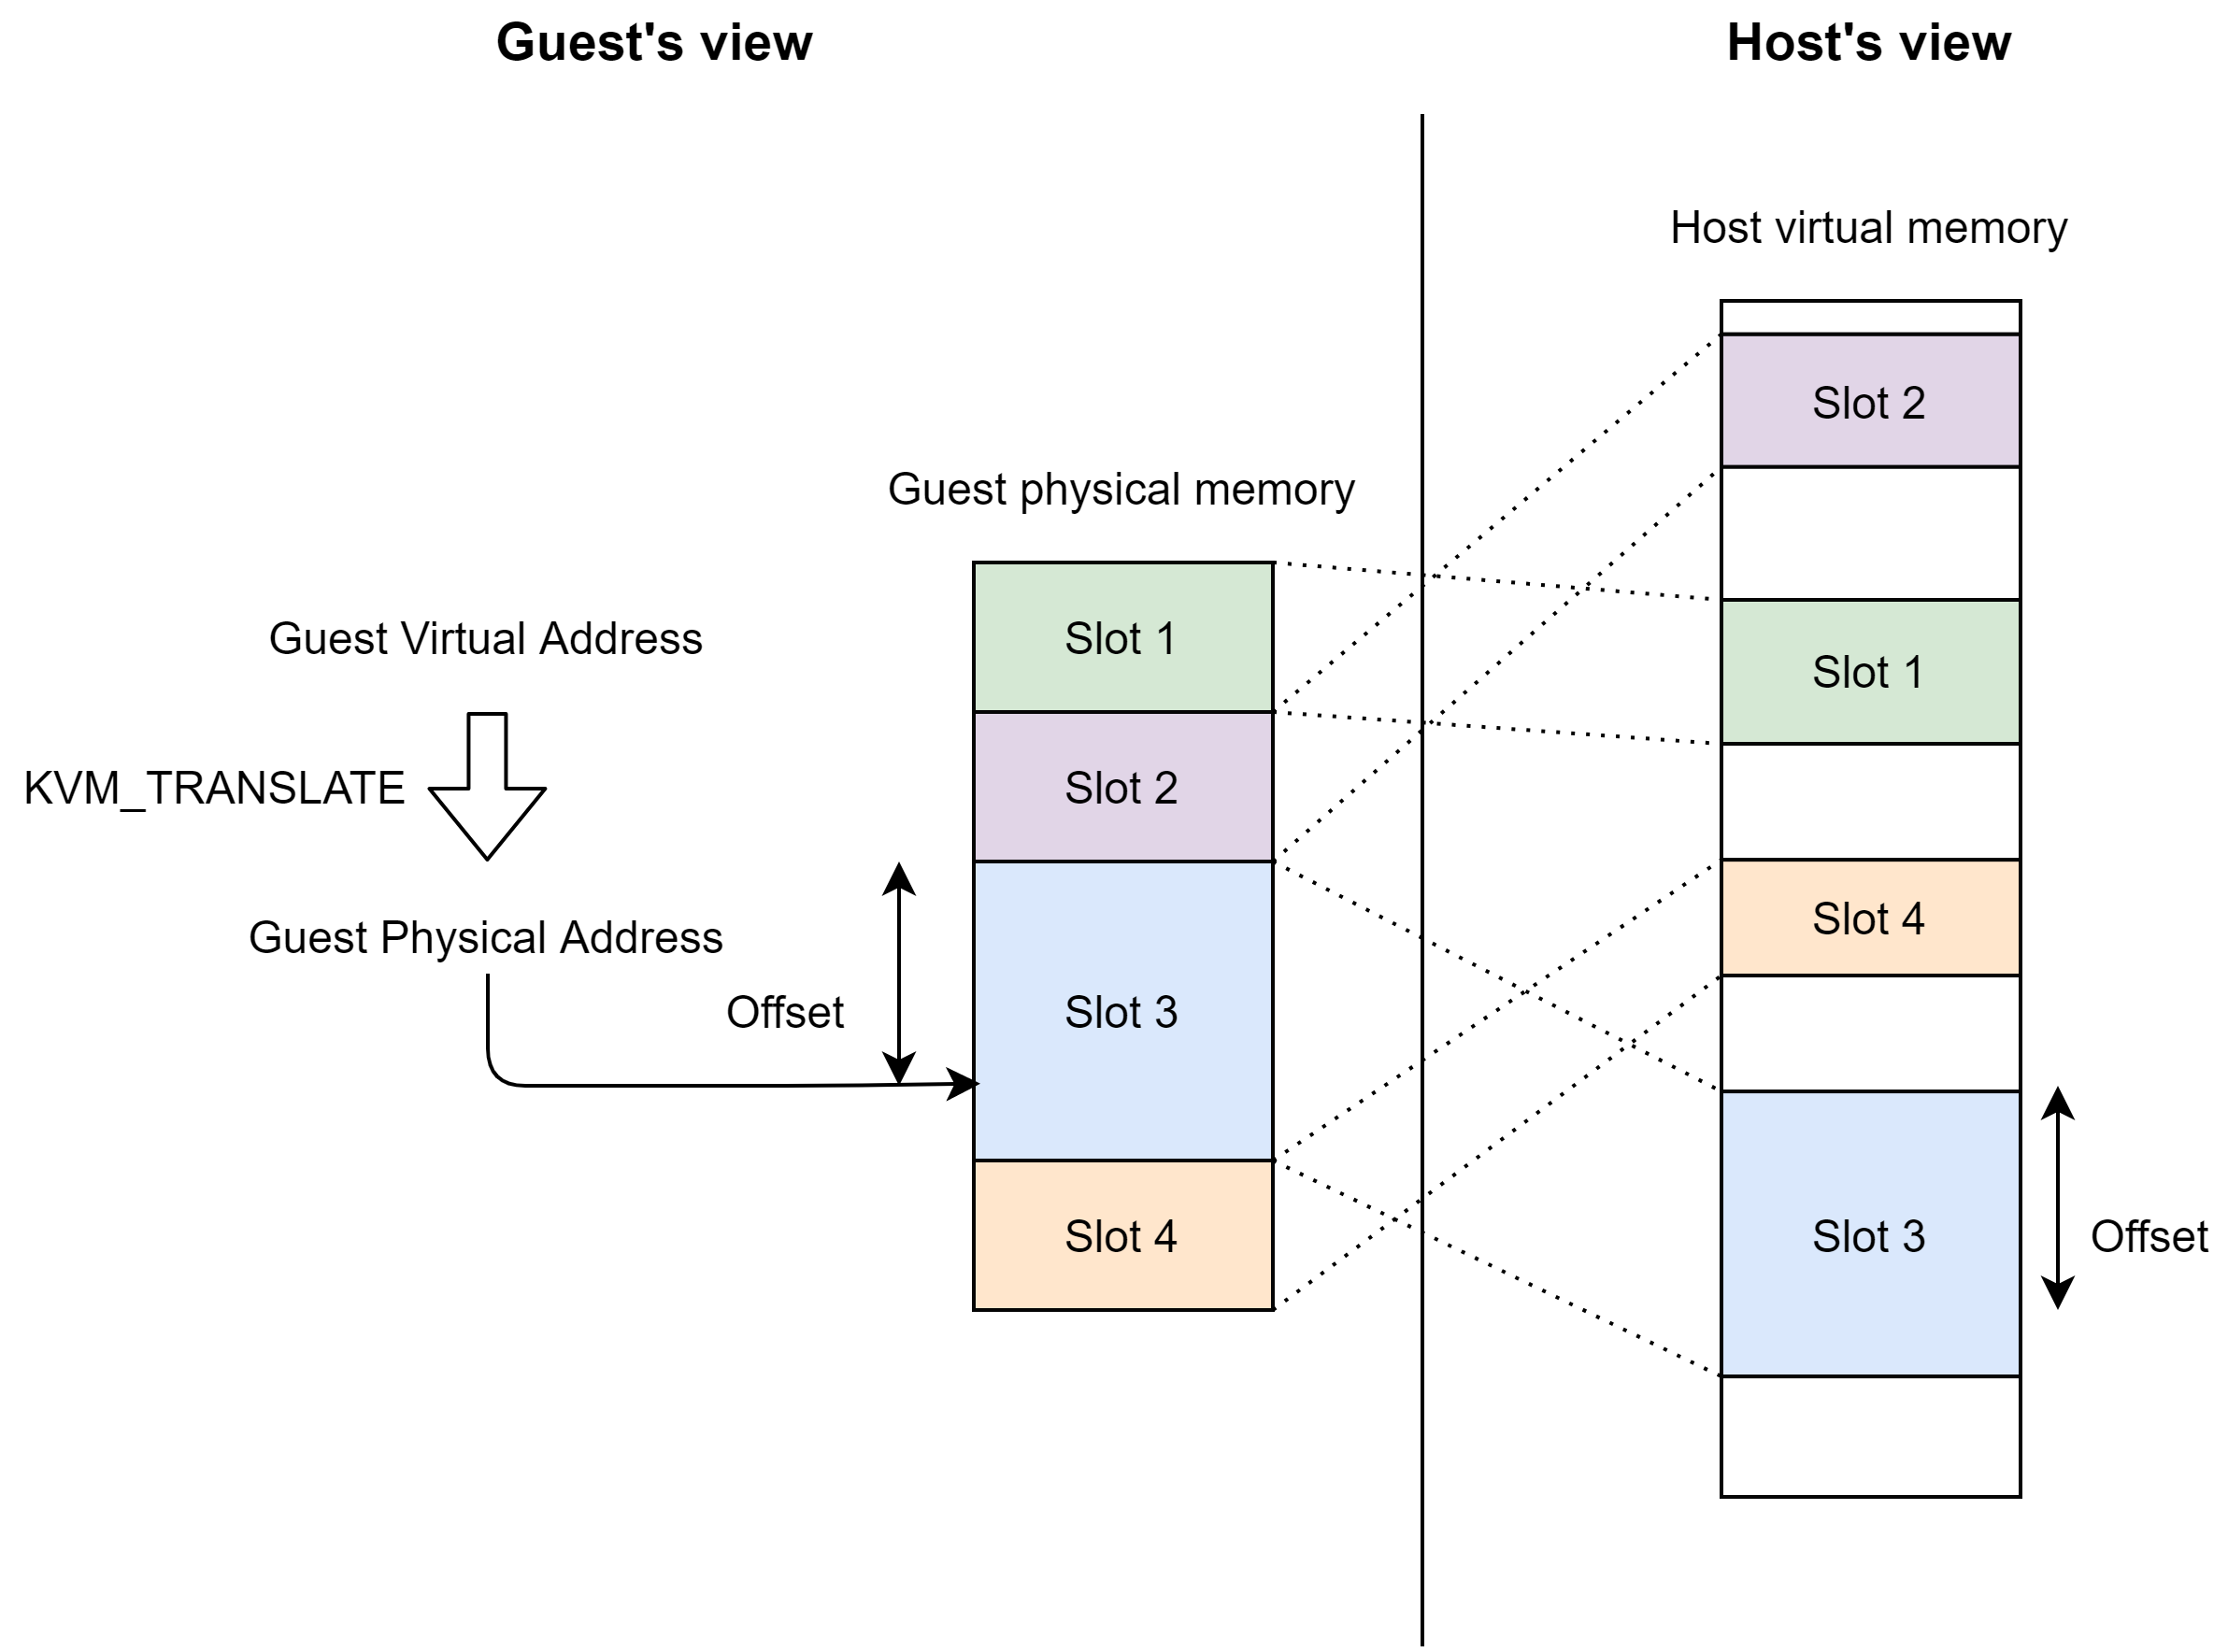
\includegraphics[width=\textwidth]{images/translation.png}
  \caption{Translation of a GVA to a HVA}
  \label{fig:translation}
\end{figure}
\begin{enumerate}
    \item Find the \texttt{KVMSlot} in QEMU containing the obtained GPA. \texttt{KVMSlot}s are maintained in an array and it is possible to iterate over them. In particular, to find the corresponding slot, it can be checked if the GPA previously obtained is within the range of addresses between the $[start\_addr, start\_addr + memory\_size]$. If this is the case, the slot was successfully found. 
    \item Now that the slot was found, it is possible to compute the offset of the address within the slot. This offset will still be valid in the host virtual space since it is true that slots can be anywhere in the host virtual memory, but the memory corresponding to the slot is contiguously allocated both in the host virtual space and in the guest physical space.
    \item The offset and the field corresponding to the host virtual address of the slot (i.e the one with the same meaning as the \texttt{userspace\_addr} in the KVM memory region structure) can be added together to obtain the HVA.
\end{enumerate}
Figure \ref{fig:translation} summarizes the steps needed for the translation and explain it graphically. This translation from GVA to HVA is useful to let the hypervisor perform operations directly in the physical memory of the guest OS and will be used as an important building block throughout this work. 

\subsection{Interrupt handling in Linux}
The interrupt handler plays a crucial role in the overall system. It is the core of the system implemented in the guest and it must be protected by the hypervisor. Before actually protecting it, it should be better explained how interrupt handling works in Linux, focusing on the data structures the Linux kernel relies on. GDB, QEMU Monitor and the Linux kernel source code were used to study the interrupt handling flow, with particular attention to the flow that leads to the execution of the interrupt handler of the FX device. 
\par 
Certainly, the handling of external interrupts takes place both in hardware and software. For what concerns the hardware, on Intel architectures, devices cannot send interrupts directly to the CPU: they are instead connected to a specific device, the I/O APIC (Advanced Programmable Interrupt Controller). Each device is connected to the I/O APIC through an IRQ line and, in turn, the I/O APIC multiplexes the interrupts to the CPU, which has only one special PIN connected to the interrupt controller. The main purpose of the APIC is to monitor the IRQ lines and to notify the CPU of the occurrence of an interrupt. If more than one interrupts occurs simultaneously, the APIC also takes care of ordering the interrupts according to a given priority. To let the CPU execute a special routine to handle the interrupt, an interrupt vector is sent by the APIC to the CPU on interrupt notification. This vector is used as an index of a particular table prepared by the kernel, the Interrupt Descriptor Table (IDT). The base address (and the size) of this table is maintained in a CPU register, the Interrupt Descriptor Table Register (IDTR). The IDT table is prepared by the Linux kernel and described by the symbol \texttt{idt\_table}, which is defined as an array of \texttt{gate\_desc} (which in turn is a \texttt{typedef} for \texttt{gate\_struct}) as shown in Listing \ref{list:idt_table}.
\begin{lstlisting}[style=c, caption={Definition of the idt\_table}, label={list:idt_table}]
static gate_desc idt_table[IDT_ENTRIES] __page_aligned_bss;

struct idt_data {
	unsigned int	vector;
	unsigned int	segment;
	struct idt_bits	bits;
	const void	*addr;
};

struct gate_struct {
	u16		offset_low;
	u16		segment;
	struct idt_bits	bits;
	u16		offset_middle;
#ifdef CONFIG_X86_64
	u32		offset_high;
	u32		reserved;
#endif
} __attribute__((packed));

typedef struct gate_struct gate_desc;
\end{lstlisting}
The memory layout of the IDT entries is completely described by the \texttt{gate\_struct}  struct. Since it is a particular memory layout, for convenience the Linux kernel uses the \texttt{idt\_data} struct, and then when it needs to actually copy the information in one of the IDT entries, it uses conversion functions to transform it into the corresponding \texttt{gate\_struct}. The segment selector field is an index into the Global Descriptor Table and, together with the offset, can be used for starting the execution of the interrupt handling part implemented in software. 
\par
The Linux kernel tries to split interrupt handling into three different levels of abstraction:
\begin{itemize}
    \item a part of the code must be architecture-dependent and must be aware of the details of the interrupt controller
    \item on top of the hardware-specific part of code, a generic IRQ handling is implemented, abstracting the underlying hardware details and separating the chip details and the real IRQ flow
    \item the third level of abstraction is then implemented to offer device driver writers an API for interacting with the interrupt handling subsystem. This is also useful to use the same driver on different platforms without code changes. One of the functions belonging to this level of abstraction was already used: it is the \texttt{request\_irq} function used by the FX driver to register the interrupt handler.
\end{itemize}
Of course, all these three levels of abstraction contribute to the handling of an interrupt and must be protected. The adopted strategy is to extract the trace of function calls that leads to the execution of the handler registered through the \texttt{request\_irq} function. To achieve this, GDB can be leveraged. Upon registration of the handler, the module inside the guest uses the \texttt{printk} function to output the address of the handler function (notice that the \texttt{\%px} format specifier is actually needed). Then, by setting a breakpoint on it, the chain of function calls can be easily obtained using the \texttt{backtrace} command. This is a starting point for studying the Linux Kernel source code following the obtained trace of functions. Listing \ref{list:backtrace} shows the trace of function calls.

\begin{lstlisting}[style=c, caption={Output of the backtrace command. The first entry is the one corresponding to the interrupt handler registered with the driver}, label={list:backtrace}]
[#0] 0xffffffffc0000205  mov $0xffffffffc00010ad, %rdi
[#1] 0xffffffff810b9518  __handle_irq_event_percpu
[#2] 0xffffffff810b965c  handle_irq_event_percpu
[#3] 0xffffffff810b96d3  handle_irq_event
[#4] 0xffffffff810bd231  handle_fasteoi_irq
[#5] 0xffffffff8101fba9  generic_handle_irq_desc
[#6] 0xffffffff8101fba9  handle_irq
[#7] 0xffffffff8101fba9  __common_interrupt
[#8] 0xffffffff81b57f26  common_interrupt
\end{lstlisting}
\par
One of the core data structures of the generic IRQ handling is \texttt{irq\_desc}. This data structure represents the descriptor for a IRQ. IRQ descriptors are kept in an array of descriptors, which is also called \texttt{irq\_desc}, as shown below. This array can be indexed with the same vector used in the lowest level of interrupt handling. For this reason, it is worthwhile to retrieve it for inspecting the interrupt descriptor associated with the FX device. This can be done as in the following steps: 
\begin{enumerate}
    \item The IRQ line associated with the device can be obtained by issuing the command \texttt{cat /proc/interrupts}
    \item Once the IRQ line is known, the command \texttt{info pic} of the QEMU Monitor shows the interrupt vector.
\end{enumerate}
Then, making use of the GDB \texttt{print} command it is possible to index the \texttt{irq\_desc} array to show the content of the interrupt descriptor. 

\begin{lstlisting}[style=c, caption={\texttt{irq\_desc} data structure (redacted) and array definition}, label={list:irq_desc}]
struct irq_desc irq_desc[NR_IRQS] __cacheline_aligned_in_smp = {
	[0 ... NR_IRQS-1] = {
        ... /* initialization redacted */
	}
};

struct irq_desc {
    ... /* redacted */
	irq_flow_handler_t	handle_irq;
	struct irqaction	*action; /* IRQ action list */
    ... /* redacted */
} ____cacheline_internodealigned_in_smp;
\end{lstlisting}
Once the fields are printed on the screen, the analysis can proceed further by examining the two of them reported in Listing \ref{list:irq_desc}. These are the most relevant fields of the \texttt{irq\_desc} data structure and also for the overall interrupt handling mechanism. The main reason is that they allow crossing the three level of abstractions. In fact, 
\begin{figure}[t]
    \centering
    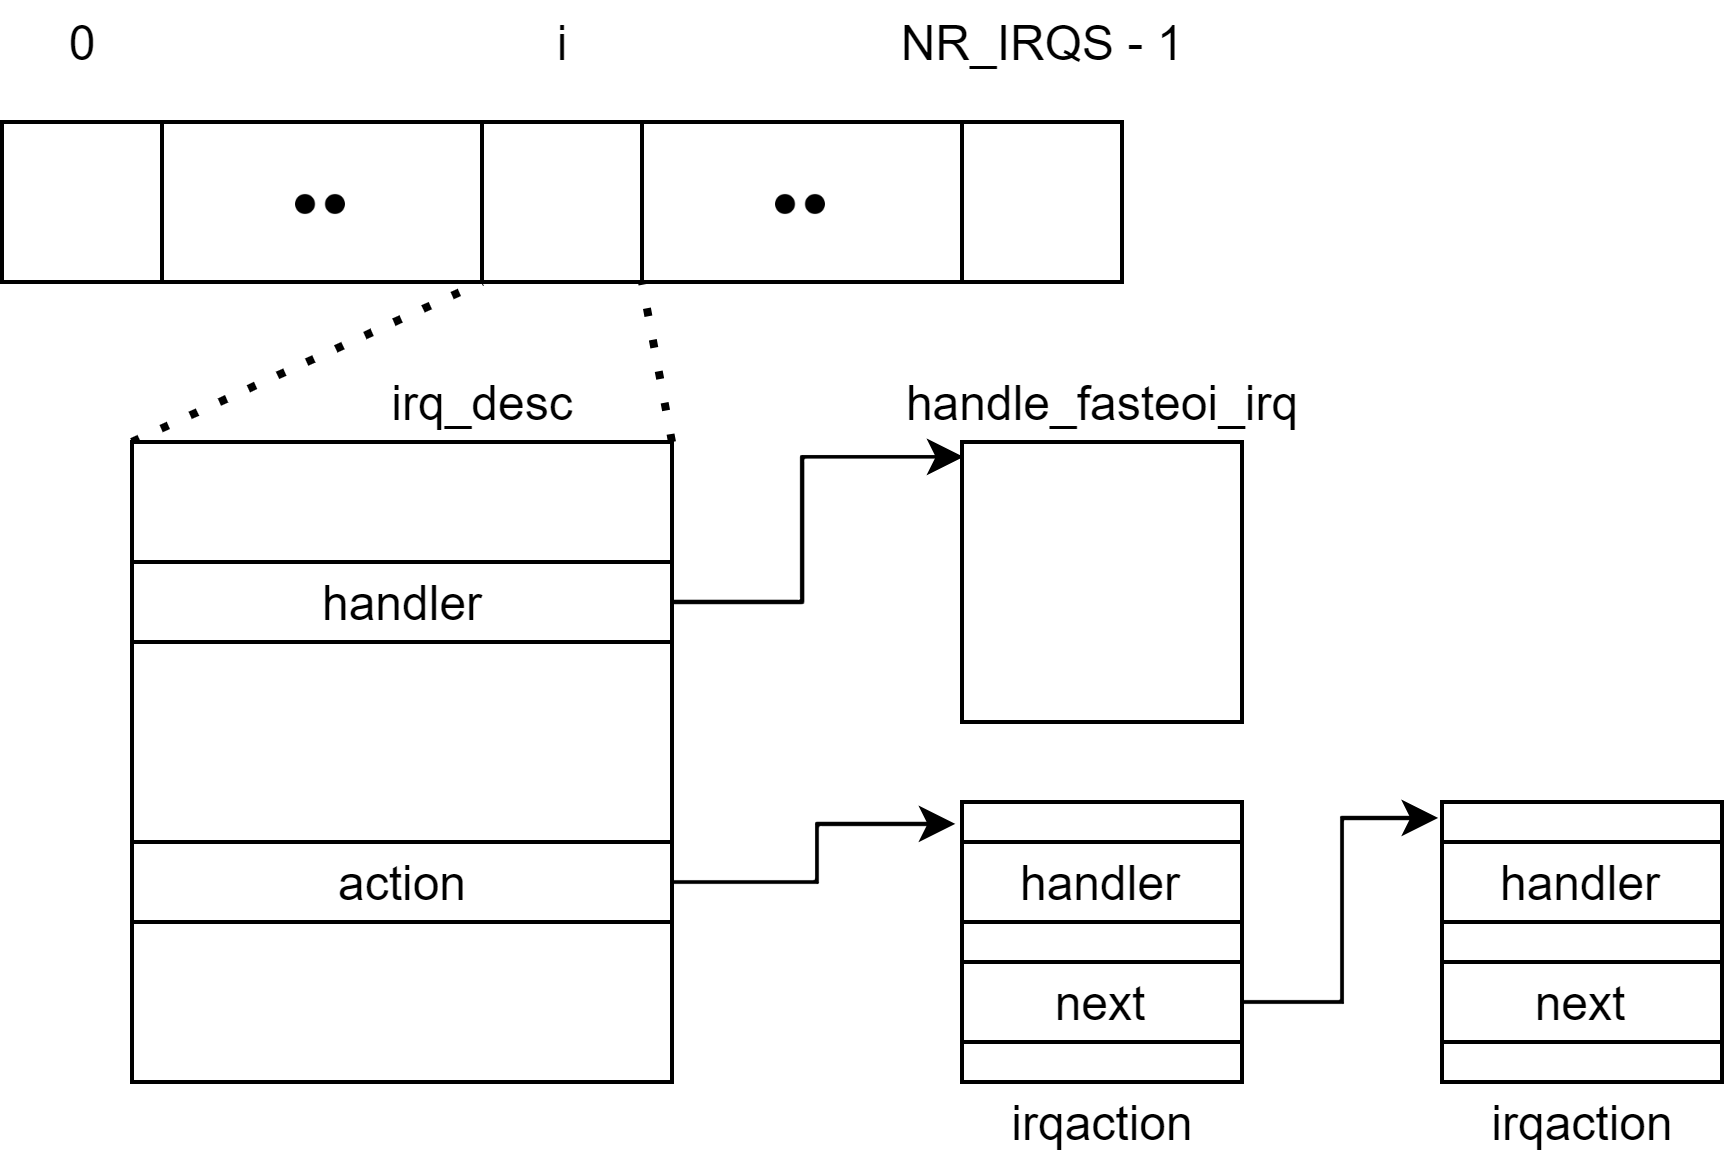
\includegraphics{images/interrupt-handling.png}
    \caption{Interrupt handling main data structures}
    \label{fig:interrupt-handling}
\end{figure}
\begin{itemize}
    \item The \texttt{handle\_irq} is a function pointer. It points to the function that must be called by the lowest level of abstraction to start the generic IRQ handling. For what concerns the interrupt related to the FX device, \texttt{handle\_irq} points to \texttt{handle\_fasteoi\_irq}.
    \item The \texttt{action} field, instead, is the head of a list of \texttt{irqaction}s. This list is used to call the handlers registered through the \texttt{request\_irq} function and, for this reason, it is used to reach the highest level of abstraction of the interrupt handling mechanism. It has to be noticed that this list is maintained to allow the sharing of an IRQ. On interrupt, the kernel calls all the handlers stored in the list of \texttt{irqaction}s. It is up to the interrupt handler to understand if it was its device that originated the interrupt.
\end{itemize}
For the sake of clarity, these important data structures and their connections are shown in Figure \ref{fig:interrupt-handling}

\par 
These were the most important concepts on how the hardware and the Linux kernel cooperate to handle an interrupt. The next section will make use of this useful information to try to protect the overall mechanism. 
\subsection{Memory protection from the hypervisor}
One way to protect the guest agent is by enforcing memory write protection from the hypervisor. Most of the background knowledge needed to protect the interrupt handler was already discussed and this section explains how the protection was implemented.
\par 
In general, two strategies can be implemented by the hypervisor:
\begin{itemize}
    \item Monitoring. Some of the kernel objects are invariant from the time the handler is installed to the time the virtual machine is shut down. The integrity of these objects can be periodically checked by the hypervisor. This is a sort of passive protection. 
    \item Write protection. The hypervisor can ensure that certain parts of memory, in particular corresponding to sensitive data structures and code, cannot be written. This is referred to as active protection. 
\end{itemize}
Whenever it is possible, active protection must be used. This is because it is better to readily stop not allowed operations instead of periodically monitoring the important kernel object. In fact, it could be the case that monitoring is not enough if the monitored object is checked periodically: the attacker could modify the object to complete the attack and then restore its state. If this happens between two consecutive checks of the monitoring code, the attacker can bypass this protection.
\par
In this case, active protection can be implemented thanks to the \texttt{KVM\_MEM\_READONLY} flag of KVM memory slots. This flag is important also because it allows to implement the protection from userspace, thus avoiding writing any code inside the KVM kernel module and not enlarge the attack surface by introducing bugs inside the host kernel. As already explained, this flag prevents any write operation to a particular memory slot, but not reads. Also, code contained in such a memory slot can be executed. If a write is issued in a slot marked as read-only, a VM Exit occurs and the hypervisor regains control of the execution. The associated exit reason will be \texttt{KVM\_EXIT\_MMIO}. To protect a specific part of memory, the following steps can be performed: 
\begin{enumerate}
    \item The slot containing the chunk of memory to be protected can be temporarily removed. This operation can be done by issuing the same ioctl used to allocate the slot but passing zero as size. As a result, the virtual machine will now miss a part of its physical memory. Notice that this part of physical memory is still reachable using the virtual address space of the hypervisor so that anything is lost because it will be remapped soon.
    \item The removed slot is then split into three parts: the chunk of memory that has to be protected is put in a slot whose size is the minimum amount of bytes needed to contain it. This slot is inserted again by computing the right physical address and associating it with the right corresponding host virtual address. The remaining part of memory belonging to the previously removed slot is allocated again, without any kind of flags. 
\end{enumerate}
\begin{figure}
\centering
  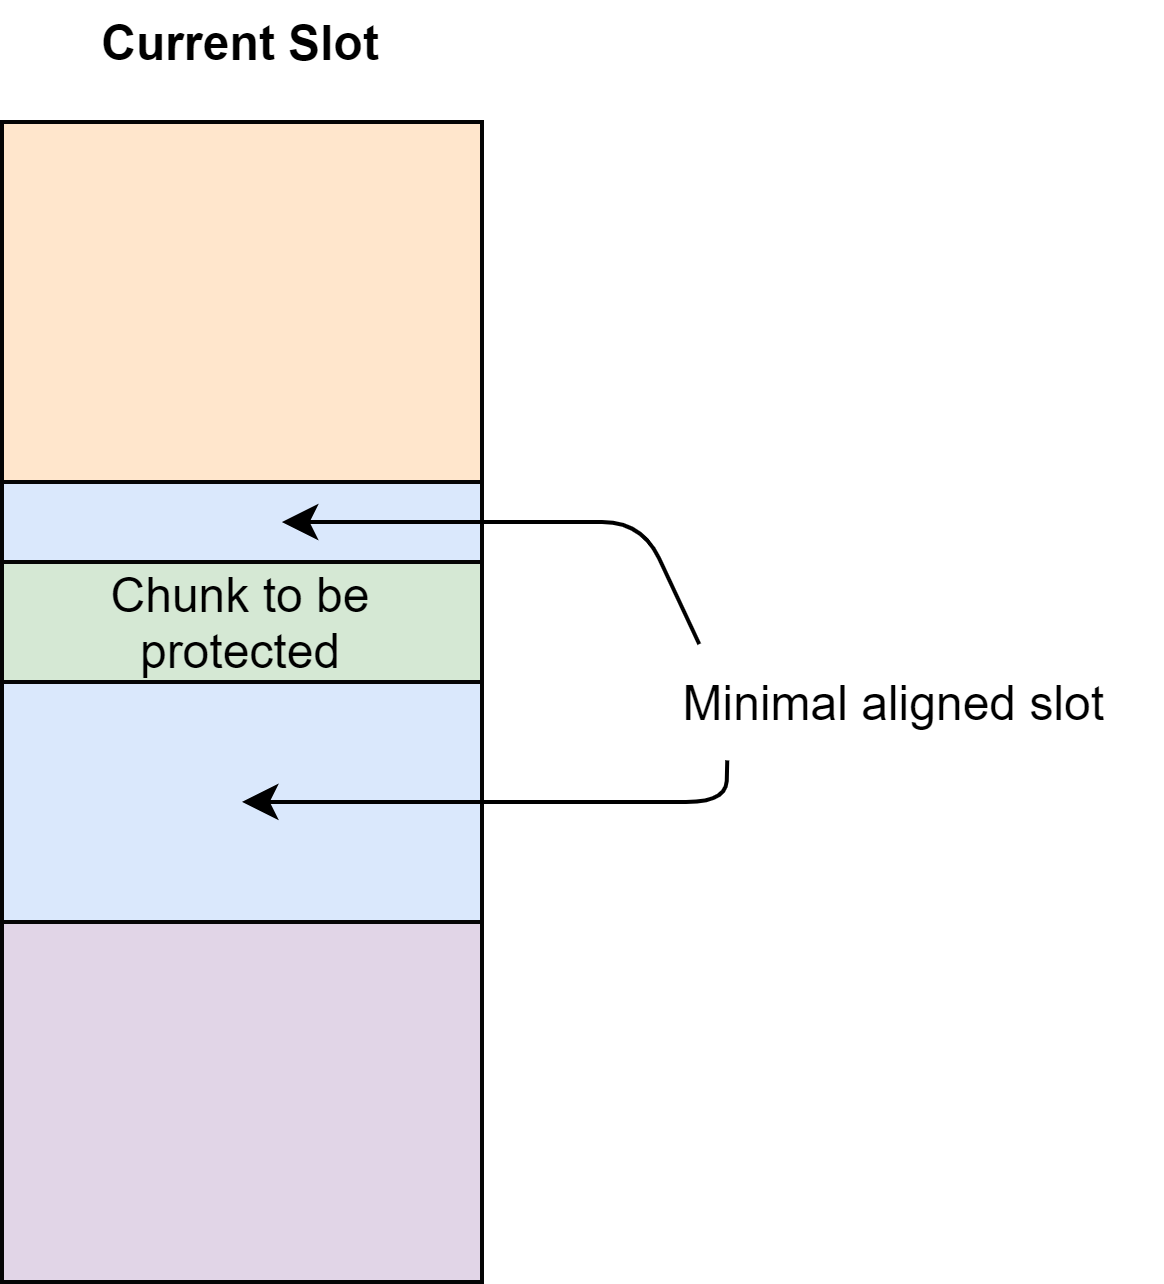
\includegraphics[scale=1]{images/slot-splitting.png}
  \caption{Slot-splitting technique. The current slot is represented by the biggest rectangle. Colors illustrate how it will be split. The green part is taken into account by the PMC data structure.}
  \label{fig:slot-splitting}
\end{figure}
Figure \ref{fig:slot-splitting} summarizes these operations. This is a completely working approach. However, it has to be noted that this slot splitting technique can operate only with page granularity, but the chunk of memory to be protected can be smaller. This is due to the fact that Intel VT-x requires that memory allocated to the guest is page aligned, so that it is possible to make use of Extended Page Tables (EPT) to virtualize the guest's MMU, as already pointed out in the introduction. 
\par 
This problem is solved by introducing a new data structure in the hypervisor, called \texttt{protected\_memory\_chunk} (PMC). The only purpose of this data structure is to protect only the specific part of memory containing sensitive information with a finer granularity. To do this, whenever the guest asks to protect a specific data structure or part of kernel code, it passes its address and size to the hypervisor. The latter will initialize a new \texttt{protected\_memory\_chunk} and will add it to a linked list. Using the data kept into each \texttt{protected\_memory\_chunk} the hypervisor can easily discriminate when the guest is trying to write in any of them, by just adding additional checks to the \texttt{KVM\_EXIT\_MMIO} exit reason. In particular, the following checks must be put in place: 
\begin{enumerate}
    \item If the write address is within a PMC, the write operation is ignored. This is an event that deserves to be logged: depending on what the PMC is containing, it could be a clue for a possible attack.
    \item If the write operation is not inside a PMC, but it is inside a slot previously created with the purpose of protecting another chunk of memory, the hypervisor performs the write on behalf of the virtual machine. To do this, the PMC struct contains a pointer to the KVMSlot crated for containing the PMC itself.
    \item All the other cases are related to normal MMIO operations, so the default behavior is used unchanged.
\end{enumerate}
\par
Another detail has to be highlighted: how the guest module can pass parameters to the hypervisor. To solve this problem without any modification to the core of KVM, a sort of custom hypercall was implemented. This is done thanks to two key observations: 
\begin{itemize}
    \item Firstly, the QEMU process can use the \texttt{KVM\_GET\_REGS} and the \texttt{KVM\_GET\_SREGS} ioctls to read all the registers of the virtual CPU. 
    \item Secondly, the QEMU process already handles the I/O emulation, thus a VM exit is triggered whenever an I/O operation needs to be executed. 
\end{itemize}
Combining these two observations, a hypercall can be implemented. The idea is to reserve a particular area of memory to let the guest call the hypervisor: this is done by reserving offset \texttt{0x80} for the BAR register already set up for the FX device. Furthermore, the guest can put variables, addresses, and sizes inside registers using extended assembly. Listing \ref{list:assembly-hypercall} shows a simple way to do that. After putting the parameters of the hypercall inside registers, the guest triggers a VM exit by writing into the BAR plus the offset designed for the hypercall. The hypervisor will recognize that the I/O operation is related to that particular port, so it will read the parameters that were previously put inside the registers and will satisfy the request. 

\begin{lstlisting}[style=c, caption={Example of hypercall: putting the base address of the loaded kernel module inside register \texttt{r8}, then triggering the VM exit}, label={list:assembly-hypercall}]
__asm__ volatile("movq %0, %%r8" 
                    :
                    :"r"(THIS_MODULE->core_layout.base));
__asm__ volatile("mov %0, %%rax" 
                    :
                    :"r"(mmio + HYPERCALL_OFFSET));
__asm__ volatile("movq $1, (%%rax)"::); /* triggering the hypercall */
\end{lstlisting}
\par 
Using the slot splitting technique together with the protected memory chunks, the hypervisor can apply protections to the overall kernel code and data structures responsible for interrupt handling and it can do it with the granularity needed, thus preventing the attacker to disable or tamper with the system residing in the guest, meeting one of the initial requirements stated in the design phase. Furthermore, it is worthwhile noticing that this memory protection can be applied to many other kernel objects. For instance, the entire .text and .rodata sections of the kernel can be protected using this approach, thus making more difficult attacks which tries to patch the kernel to execute malicious code or attacks to important read only data structures, such as the IDT or the system call table.

\subsection{Generalizing the hypercall handling}
In the previous section, it was described how the guest can ask the hypervisor to perform some operations. The result is a paravirtualized channel that can be exploited for many different purposes. For this reason, it helps to add a new parameter that can be used to distinguish different requests. This is done by introducing a \emph{type} parameter. As a consequence, the hypervisor can read this parameter by simply reading the guest register that was assigned to it and then performs actions accordingly. Furthermore, since hypercalls are similar to system calls but involves guest and host, also a custom Application Binary Interface (ABI) must be introduced. To do that, all the parameters of the hypercall are assigned to registers from \texttt{R8} to \texttt{R15}. The type parameter is of course assigned to \texttt{R8} and depending on that, the hypervisor knows which and where are all the other parameters.
\par 
Most of the introduced hypercalls are related to the protection of the agent itself or to the protection of the running kernel. It is important to notice that this newly created channel represents the opportunity to introduce many different policies and techniques to add a layer of security to the guest system, and that is the reason why it is an important achievement for this work. 
\par 
One of the most important hypercall is the already discussed memory protection hypercall. Two other different approaches that were put in place are the \emph{Save and Compare} and the \emph{Save and Reload} techniques. 
\par % save and compare
The \emph{Save and Compare} approach can be seen as a tool offered to the monitoring code and it is mainly used to let the latter analyze the state evolution of kernel data structures. This is because sometimes it could be hard to enforce only certain kind of accesses to them (such as write protection), and further analysis is needed. To implement this approach, two hypercalls are implemented. The first one is used to save a given data structure, passing its address and size to hypervisor like already described. The second one, instead, is used to compare the current state of a data structure against its saved state. The hypervisor will return back to the monitoring code the offsets in which it has detected changes in the data structure so that the guest agent can use them to semantically understand which fields were changed and to understand if something bad has occurred within the system. 
\par % save and reload
The \emph{Save and Reload} approach, instead, is used to protect the guest agent itself in an alternative way or together with the memory write protection hypercall. The key observation of this approach is that both code and data structures related to the interrupt handling mechanism must not be always protected. In fact, since the interrupts come from the virtual device in the hypervisor, the latter might need to only reload kernel objects that were previously saved when considered in a safe state. This reloading operation will be performed every time upon interrupt injection, thus forcing the guest kernel to use safe objects. This approach was also explored to reach a degree of stealthiness of the system: an attacker may try to hook function pointers or patch kernel code to execute malicious code and prevent the handler to be executed, but at the moment the interrupt is injected and managed all the kernel objects are restored in their safe state.
\par % details on save hypercall, Saved Memory Chunk
It has to be noted that both these two approaches require a hypercall to save pieces of guest memory. To do that a new data structure was introduced in the hypervisor, the Saved Memory Chunk (SMC). This data structure contains a pointer to an area of memory placed in the heap of the QEMU process which is not allocated to the VM and containing a copy of the guest memory that has to be saved. To specify if the SMC has to be used with the Save and Reload approach, a boolean flag parameter was added to the hypercall. This way, every time an interrupt of the FX device has to be injected, the hypervisor will also scan the list of SMC, checking if the flag for reloading is set. If so, the guest memory will be replaced using the previously saved memory chunk.

\par % communication channel state
Another important aspect that has to be underlined is related to the paravirtualized channel itself. This channel allows the guest agent and the hypervisor to communicate in order to implement most of the important features of the system. An attacker who already gained high privileges on the system may try to execute hypercalls to subvert the system. This, of course, needs to be denied. A simple solution is found by implementing the Finite State Machine illustrated in Figure \ref{fig:paravirt-channel}. The communication channel starts in a \emph{closed} state, in which hypercalls are simply discarded. Even more, attempts to call hypercalls in this state are also logged because they could be a clear sign of a compromised guest system. In fact, legitimate hypercalls are performed only when the communication channel is in the \emph{opened} state. The transition between these two states occurs every time the FX device raises its interrupt. When using the Save and Reload approach, all the important data structures and code of the kernel will be reloaded at this point in time, then the interrupt handler will run safely, leading to the execution of the function defined in the FX device driver. As already pointed out, the monitoring code is encapsulated in this function. From this moment, it can make use of hypercalls to communicate with the hypervisor. Since this function is executed atomically in interrupt context, no attackers can issue malicious hypercalls while the monitoring code is executing. This is true also because the system was implemented for a virtual machine running on a single vCPU\footnote{To run the system with a multiple vCPUs virtual machines the hypervisor may need to stop all but one vCPU: at the end of the day vCPU are just threads and the hypervisor already has mechanisms to kick out vCPU and regain control}. When all the needed monitoring activities are completed, the monitoring code issues a hypercall to close the channel, forcing the transition back to the closed state.

\begin{figure}[t]
    \centering
    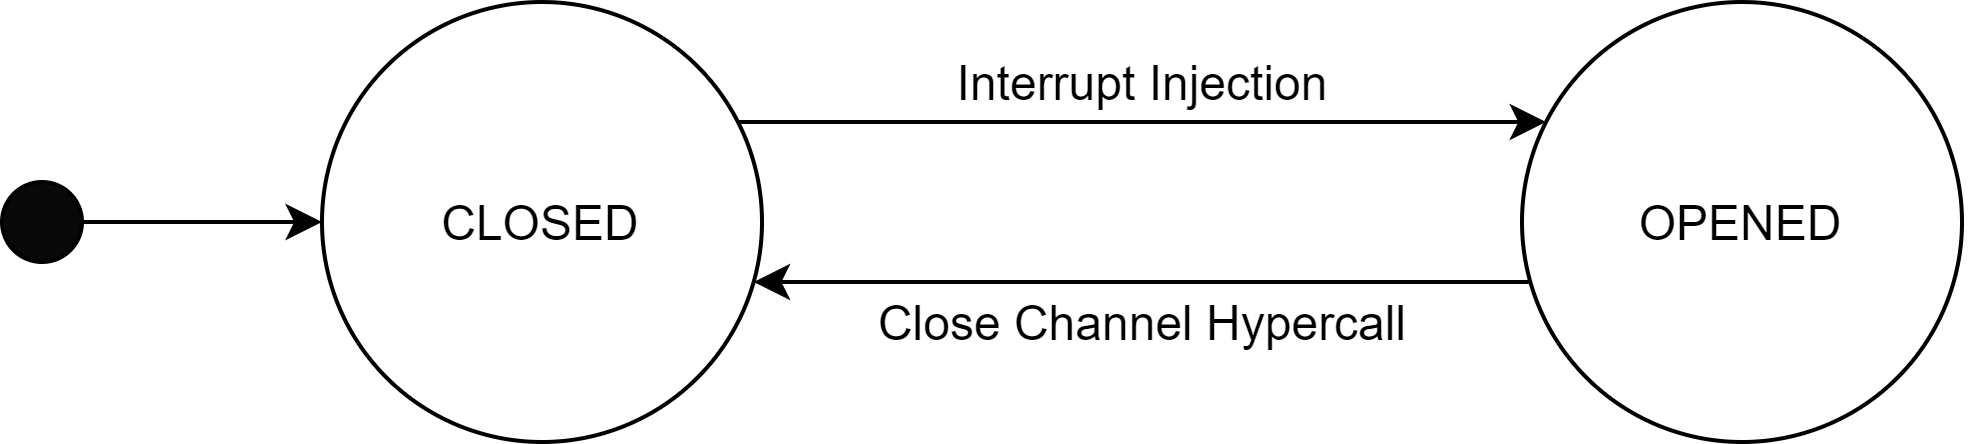
\includegraphics{images/paravirt-channel.png}
    \caption{Paravirtualized channel Finite State Machine}
    \label{fig:paravirt-channel}
\end{figure}

\par % pages for result and monitoring code state
There are also other features that the monitoring code may need to perform its work. For instance, the monitoring code may have to be stateful and return results back to the hypervisor. Furthermore, results may be too big to fit into registers. To solve these problems, the FX device drivers allocate pages in the guest system at initialization. The addresses of these pages are made known to the hypervisor through the usage of another dedicated hypercall. A part of these pages is reserved for the state of the monitoring code. This could be useful to implement, for instance, checkpointing, meaning that the monitoring code may remember where it arrived in performing its operations when it ran the last time. Checkpointing is also important because the monitoring code is running in atomic context and for performance reasons, it must try to not steal too much time from the virtual machine. The pages reserved for the state of the monitoring code are saved every time the communication channel is closed and reloaded on its opening so that an attacker cannot modify the state of the guest agent. The other part of the pages is instead reserved for results. The monitoring code makes use of these pages to pass information back to the hypervisor. The results are trusted only when the close channel hypercall is issued. In this way, results may be passed to other software tools to perform deeper analysis outside of the virtual machine. An example use case of this feature will be discussed in the following.

\subsection{Accessing all kernel symbols: the double kprobe technique}
Another important aspect that has not been considered until now is how the monitoring code can access all the symbols of the running kernel. It has to have access to all of them because it must protect the kernel internals as needed, indicating the hypervisor where important data structures reside in guest memory. This is the particular way of solving the semantic gap problem proposed in this solution.
\par The monitoring code is registered as an interrupt handler when the module is loaded. The reason why this part of the system is implemented as a module is that this solution must be usable for already compiled kernel: usually, cloud service providers install new virtual machines on demand by getting off-the-shelf images and operating systems. For this reason, the only way to add the part of the system running in the guest is by means of LKM, which are compiled independently of the core kernel. The main point is that kernel modules are supposed to use symbols that were explicitly exported. This is done to carefully select which are the variables and the functions that are considered strictly necessary to use in modules and that allow them to perform their normal operations, such as implementing device drivers. In the past, a typical workaround used by rootkits against this exporting system was found by using the \texttt{kallsyms\_lookup\_name} function. This function takes the name of a symbol as input and returns the address of it, thus allowing to programmatically know where all the symbols reside. This function is appealing also for the monitoring code, which can use it for good causes, for sure. Unfortunately, since \texttt{kallsyms\_lookup\_name} completely broke up the exporting system, it was recently unexported to make it more difficult to be used in this way. However, the unexporting of the function is not sufficient to avoid its usage, because another workaround was found, which is based on kprobes. This technique aims at using the \texttt{kallsyms\_lookup\_name} function, even if it is not exported anymore. When the address of this function is retrieved, all the other kernel symbols can be resolved by using it and that is why the target of the following method is precisely that function.
\par
As reported in the documentation, kprobes allow to dynamically break into any kernel routine and collect debugging and performance information non-disruptively. A kprobe can be registered in the system by means of the \texttt{register\_kprobe} function, which takes as input a kprobe data structure, defined in Listing \ref{list:kprobe}

\begin{lstlisting}[style=c, caption={Relevant fields of struct kprobe}, label={list:kprobe}]
struct kprobe {

    ...
    
    kprobe_opcode_t *addr;
    const char *symbol_name;
    ...

    kprobe_pre_handler_t pre_handler;
    kprobe_post_handler_t post_handler;
    ....
    
    kprobe_opcode_t opcode;
    struct arch_specific_insn ainsn;

    ...
};
\end{lstlisting}
In particular, kprobes can be attached directly to kernel addresses or symbols. To do that, the \texttt{addr} and the \texttt{symbol\_name} members can be used, respectively. It has to be noted that if the symbol's name is specified, the registering function makes use of the \texttt{kallsyms\_lookup\_name} function to retrieve the address of the symbol, and this is why kprobes become interesting. Internally, kprobes work by saving the instruction at the address specified using the \texttt{opcode} and \texttt{ainsn} members and replacing it with the \texttt{INT3} instruction \footnote{on x86\_64 architectures}. The \texttt{INT3} instruction causes a breakpoint exception, resulting in a call of the debug exception handler. When execution control is taken by the exception handler, all the CPU's registers are saved. The handler is then responsible for passing the state of the processor to the function pointed by the \texttt{pre\_handler} pointer, which is a function defined by the user of the kprobe. This function can examine the state of the processor for its own purposes. When it returns, the exception handler is responsible for emulating the instruction that was replaced by \texttt{INT3}. When it finishes, it calls the function pointed by \texttt{post\_handler}, another user-defined function. After, the exception handler let the CPU run again at the instruction next to the probed one. Now, to reach the goal of retrieving the address of the function \texttt{kallsyms\_lookup\_name}, two considerations can be made: 
\begin{enumerate}
    \item A kprobe can be placed at the address of the \texttt{kallsyms\_lookup\_name} symbol.
    \item As already pointed out if a symbol is specified instead of an address, the address of that symbol is retrieved internally by means of \texttt{kallsyms\_lookup\_name}.
\end{enumerate}
The technique to retrieve the target address can be named \emph{double-kprobe} technique: it consists on inserting two kprobes. The first one is used to replace the first instruction of the  \texttt{kallsyms\_lookup\_name} with the \texttt{INT3} instruction. Now, whenever that function gets executed, the \texttt{pre\_handler} function is called, which contains code defined in the kernel module. Then, the kernel module tries to register a second interrupt by using a second symbol name, which can be again the \texttt{kallsyms\_lookup\_name} symbol. In this way, the module indirectly calls the target function and the \texttt{pre\_handler} of the first kprobe gets executed. Now, since the state of the processor is passed to the \texttt{pre\_handler} function, it is possible to read the value of the instruction pointer, which will contain the address of the instruction next to the \texttt{INT3} instruction. Since the opcode of the latter is only one byte long, the \texttt{pre\_handler} obtains the address of \texttt{kallsyms\_lookup\_name} by just subtracting one from the value of the instruction pointer. This is the address of the target function and now, by means of that, the kernel module is now capable of accessing all kernel symbols and it is free to show the hypervisor where important data resides in memory.


\subsection{Module hiding}
The part of the system placed in the guest also tries to be invisible, at least when trying to detect its presence using simple tools. The main point is to let any user not being able to remove the kernel module with commands like \texttt{rmmod} and to not show any the entry of the module in the list of loaded modules when using \texttt{lsmod}. To do that, the main observation to do is kernel modules are kept in a list of \texttt{module} structs. By simply removing the current module from this list, the module will not appear anymore in \texttt{/proc/modules}, the directory is used for instance by \texttt{lsmod} to list all the loaded modules. Moreover, modules are also visible in the \texttt{sysfs}. To hide them there, the corresponding \texttt{kobject} could be deleted, and that is how the module was hidden inside the guest system.  Moreover, by using the Save \& Reload approach, the kernel module does not need to be in memory every time: when receiving the close channel hypercall, the hypervisor could also decide to completely delete all the code and data of the module, and reinsert them later on interrupt injection. 

\section{Customizing KVM kernel module}
The previous sections described how the system was implemented in the userspace part of QEMU and the guest operating system. To improve it, however, some work has been carried out also in the KVM kernel module. The following sections describe two new features of the system that are made possible only through the usage of the part of the hypervisor residing in the host kernel. These new features are both an improvement of the current system and a starting point for generating data for further inspecting the state of the virtual machine for security purposes. It is important to say that all the modifications of the KVM kernel module are done and thought to be relatively easy and short in terms of lines of code. This is important to not increase the attack surface of the hypervisor, and, as a consequence, to still have the assumption that the attacker cannot  directly attack the hypervisor itself.

\subsection{IDTR and Control Registers active protection}
As already explained, the Interrupt Descriptor table is one of the key data structures for interrupt handling. It is prepared by the Linux kernel and used by the hardware, which accesses it through the IDTR register. If the entry of the IDT that corresponds to the pin to which the FX device is attached or the IDTR are modified by the attacker, the overall system can be compromised. Until now, to solve this problem, the IDT table was write-protected by means of the related hypercall. The IDTR register, instead, in the first prototype of the system was checked from time to time in QEMU. In particular, the system registers are read by means of the \texttt{KVM\_GET\_SREGS} ioctl, then it was checked if the IDTR register contained a value that is equal to the one that it had when the FX device driver was installed in the system. The check was initially performed every time on VM Exit, before executing guest code again. This approach is too simplistic: the attacker can perform its operations and modify IDTR inside the window of time consisting in two VM Exit, and the hypervisor will never notice a change in the IDTR value. This is one example of why active protection is usually way more effective than monitoring.
\par 
To actually pass from a monitoring to an active protection approach, the KVM kernel module needs to be modified. Two are the key observation to implement this:
\begin{enumerate}
    \item As briefly discussed in the introduction, there exists a secondary execution control of the VMCS called \emph{Descriptor-table Exiting}. It lets the hypervisor regain control whenever the IDTR is read or written. 
    \item There must be a way to let the guest agent tell the hypervisor to enable the active protection.
\end{enumerate}
Point 1 is already a solution on its own. In fact, by simply using the \texttt{SECONDARY\_EXEC\_DESC} macro it is is possible to enable that secondary execution control. For point 2, the situation is different. The idea could be to implement a new hypercall, in the same way as before. However, if the same mechanism of the implemented hypercall is reused, the userspace part will handle it and then it cannot enable the active protection directly, because this feature is more suitable to do in the kernel part. A workaround could be to implement also a new ioctl to specifically enable this new protection. However, this is not the followed approach, since a new one was explored. In fact, another way to let the guest agent communicate with the hypervisor\footnote{this time directly with the kernel part} is to use custom MSR registers. As reported in the documentation \cite{kvm-msr}, KVM offers the opportunity to define some custom MSRs which are completely emulated by KVM itself. The idea is to define a new MSR register and initializing it with a zero value. Then, when the FX device driver is loaded, it can enable the active protection of IDTR by simply writing a non-zero value to that register. To write to specific MSR registers one can use the \texttt{native\_write\_msr} Linux kernel function, which is simply a wrapper for the \texttt{WRMSR} instruction. When a non-zero value is written into that register, the active protection is enabled and this is all the FX kernel module must do. Internally, the write is directed to a variable called \texttt{idtr\_pinned}, and precisely to a newly defined field of the \texttt{kvm\_vcpu\_arch} struct. When this variable is set to a non-zero value, all the subsequent writes are ignored, to avoid to turn the protection off by rewriting a zero value in the MSR register. Then, by simply adding an \texttt{if} statement to the \texttt{emulator\_set\_idt} function defined in the x86.c file, it is possible to check whether \texttt{idtr\_pinned} contains a value different from zero. If so, the function returns without setting the IDTR register. Since all attempts to write the IDTR register end up in a call to this function because of the activation of the Descriptor-table Exiting secondary execution control, the guest cannot modify the IDTR register anymore during its execution, thus achieving what was the initial goal.
\par 
It is interesting to notice that this mechanism can also be applied to other relevant registers to implement further protections, not strictly related to the guest agent but to the running guest kernel. For instance, other protections that were implemented involve the CR0 and CR4 control registers. A control register is a processor register which changes or controls the general behavior of a CPU. Usually, each bit of the register are used to enable or disable certain features, and that is the difference with the IDTR register, which instead contains an address (and the size) of the IDT. To deal with them, the pinning of certain bits was implemented. It consists in forcing that only certain bits, once pinned, cannot be flipped. To implement this mechanism a slightly different approach was used. In particular, for each control register two custom MSRs are defined. The first one only supports reading operations and is used to tell the device driver which bits can be pinned. The other one, instead, is used to actually pin the bits. As in the example of the IDTR register, this latter MSR starts with a value of 0 and only allows writes that set the bits allowed, specified in the read register as just discussed. As usual, to complete the active protection there is the need to control the guest exiting and to add some logic to the functions that KVM internally uses to set bits in these registers. To be precise, the way the hypervisor regains control is by means of the Guest/Host Masks and Read Shadows for CR0 and CR4 as reported in the Intel documentation. To add the new logic concerned with pinning certain bits of these control registers, the related functions are \texttt{kvm\_set\_cr0} and \texttt{kvm\_set\_cr4}. This allowed to introduce a paravirtualized version of the control register pinning inserted in the Linux kernel by Kees Cook and briefly described here \cite{kees-cook}. There are many other registers and bits that can use these ideas to protect the running kernel. Tests were performed with the CR0.WP and CR4.SMEP bits, which are a typical target of rootkits and exploits, but a similar protection could be implemented to protect the entry point of system calls (LSTAR MSR) and the bit that turns on the No-Execute protection (EFER.NXE), for instance.

\subsection{Implementation of an Access Log in KVM}
Many other features of the system could be implemented by modifying the KVM kernel module, but there is one in particular that deserved to be explored and implemented. Also, implementing this allows to pave the way for implementing many other approaches in a fairly similar way. 
\par
As mentioned earlier in Chapter \ref{chap:background}, in Intel hardware-assisted virtualization, the processor makes use of a second level page table to virtualize the guest MMU, which is called EPT in Intel terminology. The idea is to use the bits of the entries of the second level page tables to enforce certain kind of policies in the guest system or to monitor its behaviour. To explore this opportunity, a deep dive in the KVM code concerned with the management of the second level page tables was needed.  Recently w.r.t the time of writing, Google researchers have introduced in the mainline KVM a new way to make use of the hardware features for virtualizing the guest MMU, and they called it Two Dimensional Paging (TDP) MMU \cite{tdp-mmu}. This newly introduced part of code is much more cleaner than the old implementation and that is why the implemented system makes use of it. One of the main problems to solve is to use the EPT bits is to iterate over the second level page tables. To do that, the key data structure to use is the \texttt{tdp\_iter} struct, as shown in Listing \ref{list:tdp-iter}. When used together with the \texttt{for\_each\_tdp\_pte} it is possible to access down to the 4K page table entries, where it is possible to set or unset bits like Read, Write, Execute, Accessed and Dirty bits, as defined by the Intel documentation. 

\begin{lstlisting}[style=c, caption={\texttt{tdp\_iter} struct and related macros}, label={list:tdp-iter}]
struct tdp_iter {

	gfn_t next_last_level_gfn;
	gfn_t yielded_gfn;
	tdp_ptep_t pt_path[PT64_ROOT_MAX_LEVEL];
	tdp_ptep_t sptep;
	gfn_t gfn;
	int root_level;
	int min_level;
	int level;
	int as_id;
	u64 old_spte;
	bool valid;
};

#define for_each_tdp_pte_min_level(iter, root, root_level, min_level, start, end) \
	for (tdp_iter_start(&iter, root, root_level, min_level, start); \
	     iter.valid && iter.gfn < end;		     \
	     tdp_iter_next(&iter))

#define for_each_tdp_pte(iter, root, root_level, start, end) \
	for_each_tdp_pte_min_level(iter, root, root_level, PG_LEVEL_4K, start, end)

\end{lstlisting}
The \texttt{tdp\_iterator} will perform a pre-order traversal of the paging structure towards the mapping of the \texttt{next\_last\_level\_gfn} guest frame number. In particular, it is possible to set the minimum level the iterator should iterate over thanks to the \texttt{min\_level} field. The \texttt{level} field, instead, contains the level in the paging structure where the iterator is currently on. Other two particularly relevant fields are \texttt{sptep} and \texttt{old\_spte}, which are a pointer to the current descriptor and a snapshot of the value contained in it, respectively. Through the usage of the \texttt{spte} pointer it is possible to actually set or unset bits in the descriptor. To reach the goals of this work, only 4KB page descriptors were modified. Finally, another important field is the \texttt{valid} one, which can be used to assess whether the iterator walked off the end of the paging structure.
\par 
For the purposes of this work, a good candidate bit to use as an example is the Access bit. This bit is automatically set by the hardware when the corresponding guest physical page is accessed, both in read and write operations. Currently, the KVM API only supports a set of ioctls for dirty logging, but no access log is implemented. The idea is to actually implement it, so that other software tools can use it to implement further monitoring activities in the system. The design of the new ioctls used to start logging and to retrieve the log are pretty similar to the ones related to dirty logging. Specifically, the two new ioctls are: 
\begin{itemize}
    \item \texttt{KVM\_CLEAR\_ACCESS\_LOG}: this ioctl is used to iterate over all guest page descriptors to reset the access bit. 
    \item \texttt{KVM\_GET\_ACCESS\_LOG}: this ioctl takes as input a memory slot id and then it returns a bitmap array, where each of the bits correspond to a page and it is set to one if and only if that page was accessed.
\end{itemize}
There are many use cases that may be implemented using this new feature. For instance, when used in conjunction with the dirty log ioctls, the access log ioctls can be used to determine which are the pages that were accessed by read operations. Moreover, the access log was really useful to understand which pages were accessed when handling the interrupt of the FX device and to make sure that everything was actually protected. Another relevant example could be the implementation of a sort of \emph{verifier} for kernel modules: the FX kernel modules could ask the hypervisor to clear the access log when a new module is being inserted in the system. The hypervisor will then be told to retrieve it after the module was loaded. By inspecting the set of accessed pages, the latter can try to understand and decide whether to trust or not the loaded module. These are just few basic examples and use cases related to the access log, but were not implemented, because the main objective of this part of work was to try to make use of the second level page tables bits.
\par 
The same reasoning and almost the same code can be reused to make use also of the Execute bit of the second level page tables, which can be used to impose further constraints to the guest system also for security purposes.

\section{A simple use case: processes, files and networking monitoring}
This section is dedicated to a brief description of what the monitoring code can actually do. As already described at the beginning of this chapter, this system tries to comply with a defense in depth approach. The monitoring code is responsible for the security of userspace applications. To monitor what is going on inside the guest system, one of the most used forensics tools can be reimplemented also in the proposed solution: process monitoring. To do this in a trustworthy way, the guest agent will use kernel information to monitor userspace processes. This is because the guest userspace cannot be trusted at any time, since compromising it is the first step of the attacker. In addition, retrieving information from the kernel and not from userspace tools help to deal with userspace rootkit. This helps to comply with the defense in depth approach. Furthermore, the system tries to protect itself and to be resilient to kernel side attacks, as discussed in the following.
\par 
Monitoring processes inside the guest system is one of the most explored ways to understand if everything is running as expected within the system and to discover malware or signs of intrusion. Many different approaches were implemented in the past. Virtual Machine Introspection techniques deserves particular attention to this discussion. Many of the VMI approaches relies on the knowledge of the offsets of the \texttt{task\_struct}'s fields, which is the Linux process descriptor. However, since the Linux kernel is constantly evolving, it may be the case that systems developed with this idea in mind are not properly working anymore after a new kernel release. Furthermore, in modern Linux kernels, important data structures have a randomized layout \cite{struct-layout-rand}: typically, the compiler lays out in memory the fields of a C structure in order of declaration, but in modern kernels the layout in memory of these structs is automatically randomized. This is done to make exploits that rely on overwriting an exact field of a C structure much more difficult. As it could be imagined, this is also an important complication that VMI techniques have to take into account to retrieve the list of processes of the running virtual machine.

\par 
In the proposed system, instead, things are much more easier. As long as the guest agent is protected, the monitoring code can use all kernel functions and data structures to retrieve not only the list of processes, but also which files were opened and which sockets are in use. Figure \ref{fig:process-list} briefly describe how that is achieved.
\begin{figure}[t]
    \centering
    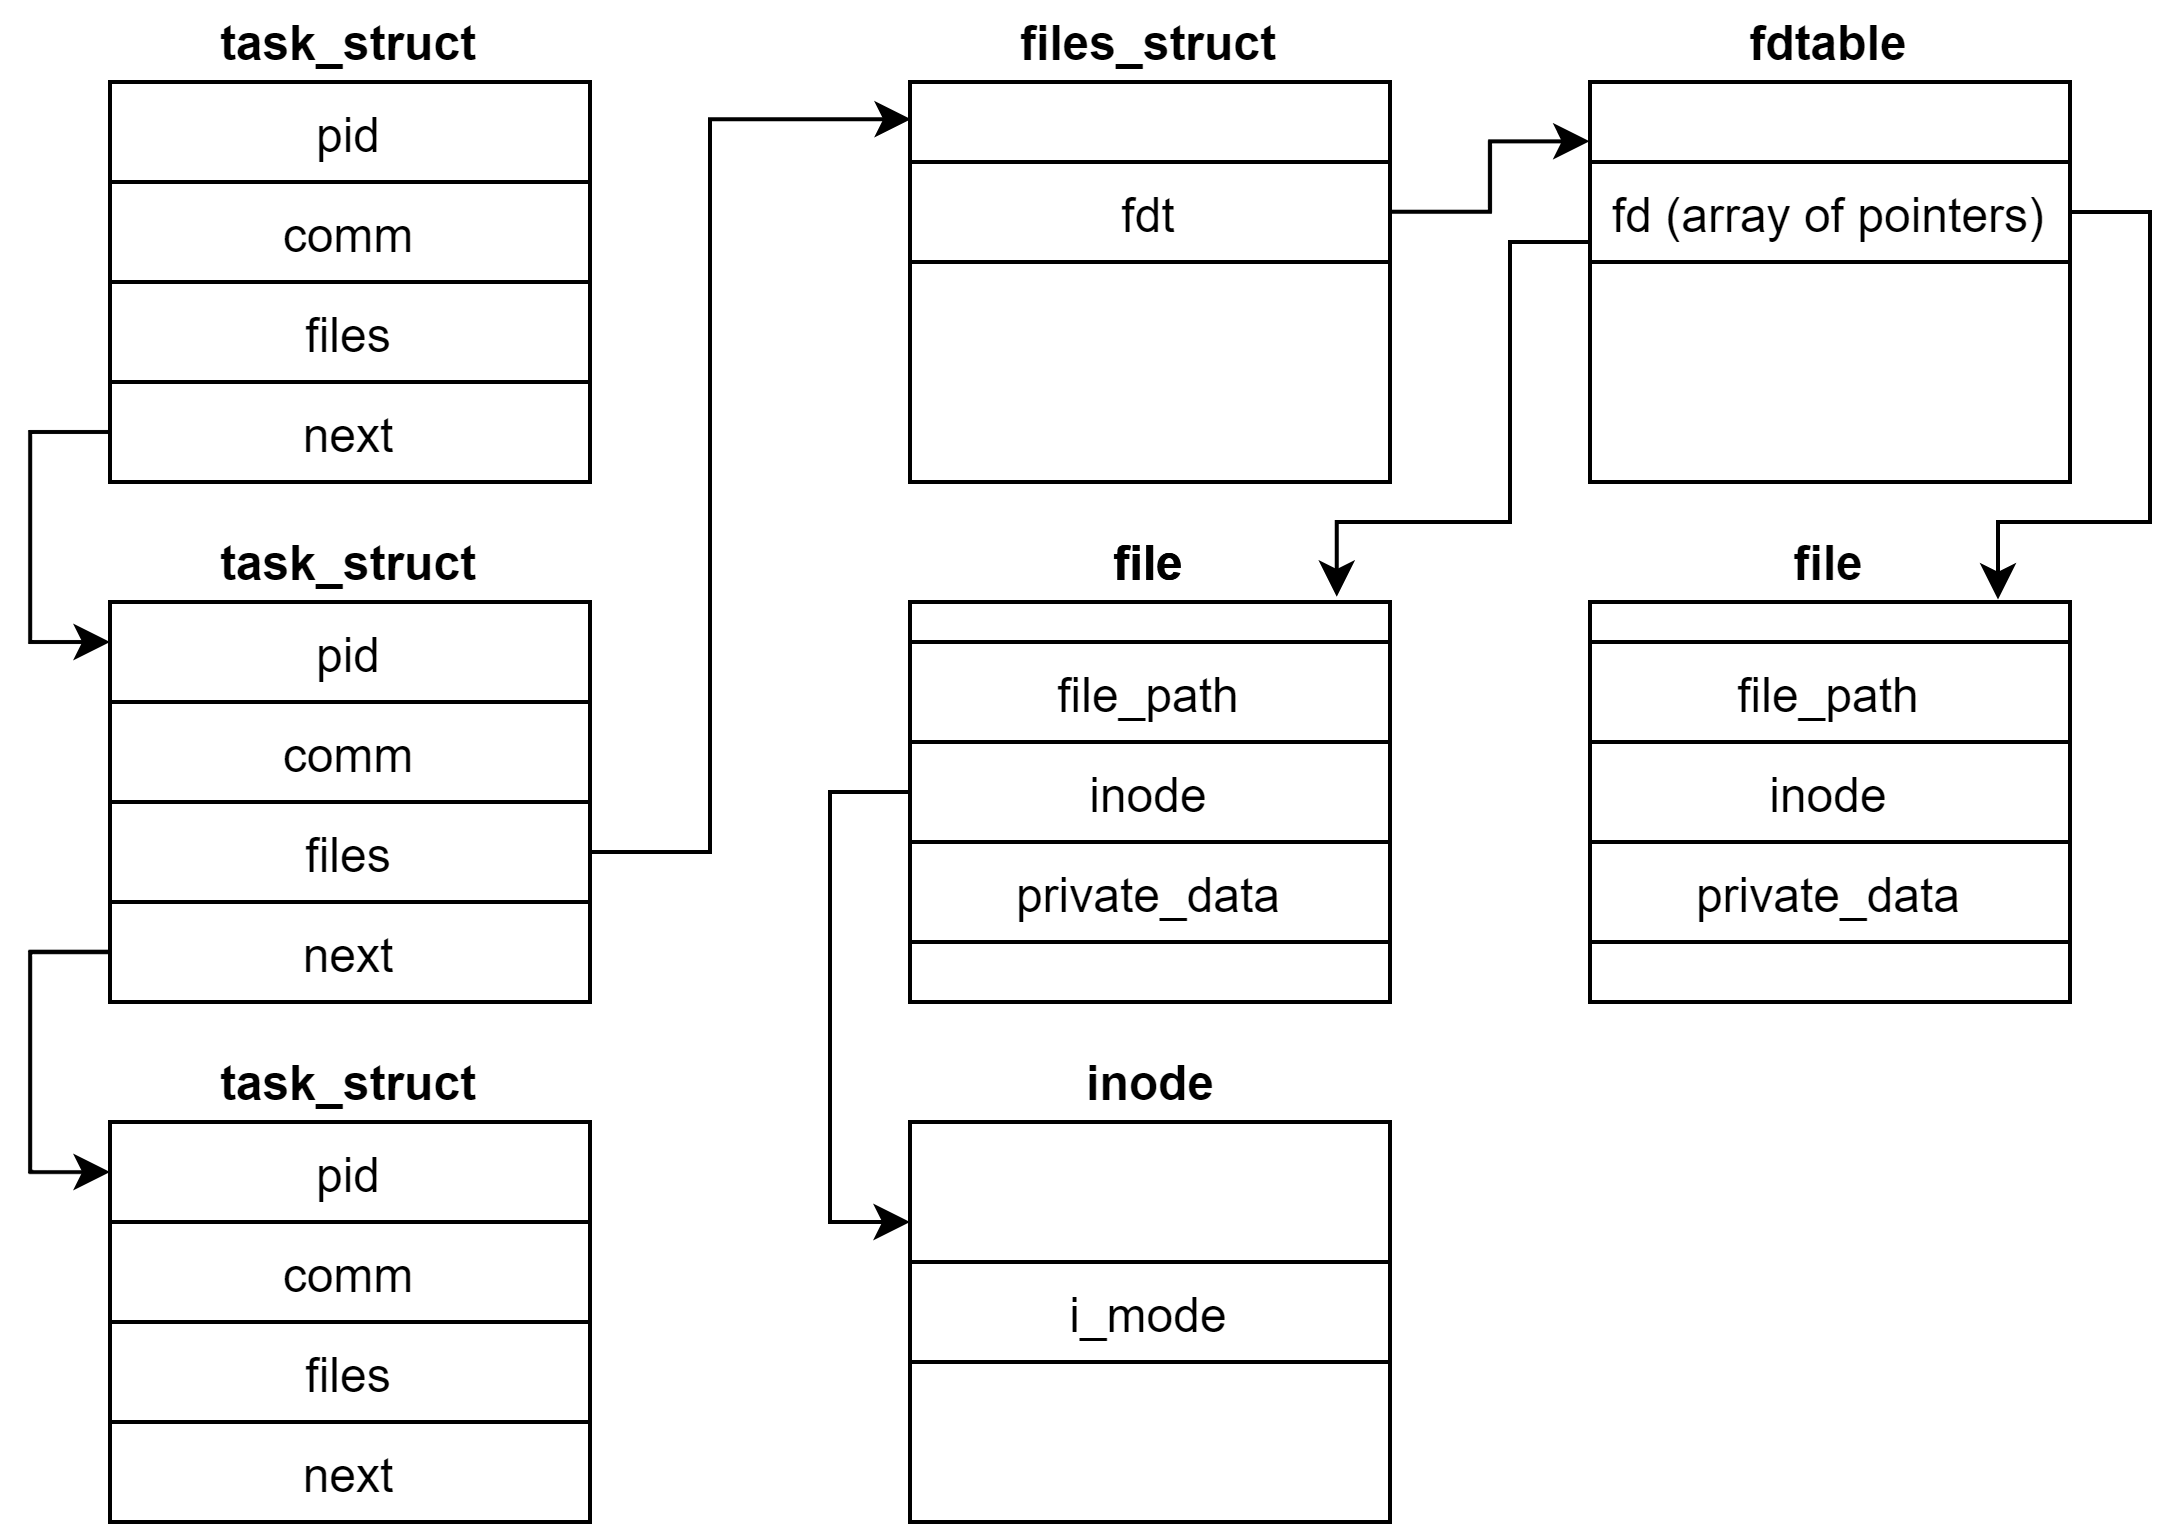
\includegraphics[]{images/process-list.png}
    \caption{Main data structures for process, files and networking monitoring}
    \label{fig:process-list}
\end{figure}
As already mentioned, the process descriptor in Linux is described by the \texttt{task\_struct} structure. Process descriptors are kept in a doubly linked list, thus it is easy to iterate over it and retrieve useful data on each process. To actually iterate over it, the \texttt{for\_each\_process} macro can be used, starting the iteration from the \texttt{init\_task}. From there, it is possible to generate a first simple output by using the \texttt{pid} and the \texttt{comm} field of each process descriptor, containing the process identifier and the command name associated with the process. Digging deeper in the fields of the \texttt{task\_struct} it is possible to identify those that are the key data structure to inspect the file descriptors of each process. Particular attention must be paid to \texttt{file} and \texttt{inode} structs. From the process descriptor it is possible to follow the \texttt{files} and the \texttt{fdt} pointers, which are pointers to \texttt{files\_struct} and \texttt{fdtable}, respectively. The actual table of opened file can be accessed through the \texttt{fd} field of the \texttt{fdtable} struct, which is an array of pointers to \texttt{file} data structures. The latter is one of the most important data structure in the Linux kernel. It represents an open file in the system. In fact, every opened file has an associated structure of this type in kernel space. The \texttt{file} structure has many important fields, among which the \texttt{f\_path}, containing the path in the file system of the opened file, and a pointer to the corresponding \texttt{inode} structs. An \texttt{inode} represents the actual file on the disk and it is important to retrieve the associated data. For the purposes of this work, the \texttt{i\_mode} can be used to understand if the file is a socket. If this is the case, the corresponding \texttt{private\_data} field inside the \texttt{file} struct pointing to that inode contains pointers to networking related data structure (specifically the \texttt{socket} and \texttt{sock} data structures). From there, it is possible to understand, for instance, if the socket is used for a TCP connection and which port is using. Listing \ref{list:proc} shows an example of the results obtained extracting data from the discussed data structures.
\begin{lstlisting}[style=c, caption={Processes, files and networking listing}, label={list:proc}]
apache2 [205]
    fd 0	/dev/null
    fd 1	/dev/null
    fd 2	/var/log/apache2/error.log
    fd 3	socket, source addr 0.0.0.0, source port 80
    fd 4	pipe:[10944]
    fd 5	pipe:[10944]
    fd 6	/var/log/apache2/other\_vhosts\_access.log
    fd 7	/var/log/apache2/access.log
bash [211]
    fd 0	/dev/ttyS0
    fd 1	/dev/ttyS0
    fd 2	/dev/ttyS0
\end{lstlisting}
As it can be noticed from the above Listing, for instance, there is an Apache 2 web server and a bash running inside the virtual machine, with PID 205 and 211, respectively. The web server is listening for incoming connections on port 80, as it can be seen from file descriptor 3. The bash process, instead, has its stdin, stdout and stderr directed to a terminal. 
\par
A few other aspects need to be highlighted. First of all, as already discussed, all the results and data collected by the monitoring system are passed to the hypervisor through the pages of guest memory allocated at initialization. The hypervisor will trust and collect the content of those pages only at the moment the communication channel goes to the closed state. Moreover, it has to be noted that the monitoring code is using internal kernel functions and symbols to perform its work. To be sure that it is using code and data structures that are not maliciously modified by an attacker within the guest system, all of them are either protected through the memory write protection hypercall or reloaded using the Save and Reload approach. Last but not least, it has to be considered that also the guest page tables and the entries related to the symbols used by the monitoring code must be protected. Again, this problem was solved thanks to the Save and Reload approach: all the translations of the kernel symbols needed by the guest agent are retrieved at the initialization through the usage of \texttt{pgd\_offset}, \texttt{p4d\_offset}, \texttt{pud\_offset}, \texttt{pmd\_offset} and \texttt{pte\_offset\_kernel} functions, then they are saved and reloaded as already discussed. This is crucial to ensure that the monitoring code is not misled by attackers that tries to manipulate the guest page tables with malicious intentions. As a result, the monitoring code is safe and its result are reliable even if the attackers has already attacked the system.